\documentclass[main.tex]{subfiles}
\begin{document}

\chapter{Continu\"iteit voor functies van $\mathbb{R}$ naar $\mathbb{R}$}
\label{cha:cont-in-r}

\section{Het continu\"iteitsbegrip}
\label{sec:het-cont}


\begin{de}
  Zij $f$ een functie en $a\in A$:
  \[ f:\ A \subseteq \mathbb{R} \rightarrow \mathbb{R}:\ x \mapsto f(x) \]
  We noemen $f$ \term{continu} in $a$ als en slechts als het volgende geldt:
  \[ \forall \epsilon \in \mathbb{R}_{0}^{+}:\ \exists \delta \in \mathbb{R}_{0}^{+}:\ \forall x\in A:\ |x-a| < \delta \Rightarrow |f(x) -f(a)| < \epsilon \]
  We noemen $f$ \term{continu} op $A$ als $f$ continu is in elke $a\in A$.
\end{de}


\begin{vb}
  De functie $f$ is continu:
  \[ f:\ \mathbb{R} \rightarrow \mathbb{R}:\ x \mapsto x^{2} \]

  \begin{proof}
    Kies een willekeurige $a \in \mathbb{R}$.
    Voor elke $x\in \mathbb{R}$ geldt het volgende:
    \[ |f(x)-f(a)| = |x^{2}-a^{2}| = |x-a||x+a| \le |x-a|(|x|+|a|) \]
    Voor $|x-a|$ kleiner dan $1$ zal $|x| \le |a|+1$ gelden.
    \[ |f(x)-f(a)| \le (2|a|+1)|x-a| \]
    Kies een willekeurige $\epsilon \in \mathbb{R}_{0}^{+}$ en kies $\delta = \min\left\{ 1, \frac{\epsilon}{2|a|+1} \right\}$.
    Uit $|x-a|< \delta$ volgt nu het volgende.
    \[ |f(x)-f(a)| < (2|a|+1)\delta \le (2|a|+1)\frac{\epsilon}{2|a|+1} = \epsilon \]
    $f$ is dus continu in $a$.
  \end{proof}
\end{vb}

\begin{vb}
  De functie $f$ is continu:
  \[ f:\ \mathbb{R}_{0} \rightarrow \mathbb{R}:\ x \mapsto \frac{1}{x} \]
  
  \begin{proof}
    Kies een willekeurige $a \in \mathbb{R}_{0}$.
    Voor elke $x \in \mathbb{R}_{0}$ geldt het volgende:
    \[ |f(x)-f(a)| = \left|\frac{1}{x}-\frac{1}{a}\right| = \frac{|x-a|}{|x||a|} \]
    Voor $|x-a|$ kleiner dan $\frac{1}{2}|a|$ zal $|x| > \frac{1}{2}|a|$ gelden.
    \[ |f(x)-f(a)| \le \frac{2}{|a|^{2}}|x-a| \]
    Kies nu een willekeurige $\epsilon \in \mathbb{R}_{0}^{+}$ en kies $\delta = \min\left\{ \frac{1}{2}|a|, \frac{\epsilon|a|^{2}}{2} \right\}$.
    Uit $|x-a|< \delta$ volgt nu het volgende.
    \[ |f(x)-f(a)| < \frac{2}{|a|^{2}}\delta \le \frac{2}{|a|^{2}}\frac{\epsilon|a|^{2}}{2} = \epsilon \]
    $f$ is dus continu in elke $a\in \mathbb{R}_{0}$.
  \end{proof}
\end{vb}

\begin{vb}
  De functie $f$ is continu:
  \[ f:\ \mathbb{R} \setminus \{-1\} \rightarrow \mathbb{R}:\ x \mapsto \frac{1}{1+x} \]

  \begin{proof}
    Kies een willekeurige $a\in \mathbb{R}\setminus \{-1\}$.
    Voor elke $x\in \mathbb{R}\setminus \{-1\}$ geldt het volgende:
    \[ |f(x)-f(a)| = \left| \frac{1}{1+x}-\frac{1}{1+a} \right| = \left| \frac{(1+a)-(1+x)}{(1+x)(1+a)} \right|  = \frac{|x-a|}{|1+x||1+a|} \]
    Voor $|x-a|$ kleiner dan $|1+a|$ geldt nu het volgende:
    \[ |1+x| = |1+a-a+x| = |1+a+x-a| \le |1+a|+|x-a| \le 2|1+a| \]
    \[ |f(x)-f(a)| \le  \frac{1}{3|1+a|^{2}}|x-a| \]
    Kies nu een willekeurige $\epsilon \in \mathbb{R}_{0}^{+}$ en kies $\delta = \min\left\{ |1+a|,3\epsilon|1+a|^{2}\right\}$
    Voor $|x-a| < \delta$ geldt dan het volgende:
    \[ \frac{1}{3|1+a|^{2}}|x-a| < \frac{1}{3|1+a|^{2}}\delta \le \frac{3\epsilon|1+a|^{2}}{3|1+a|^{2}} = \epsilon\]
    $f$ is dus continu in elke $a \in \mathbb{R}\setminus \{-1\}$
  \end{proof}
\end{vb}

\begin{vb}
  De functie $f$ is continu:
  \[ f:\ \mathbb{R}^{+} \rightarrow \mathbb{R}:\ x \mapsto \sqrt{x} \]

  \begin{proof}
    Kies een willekeurige $a \in \mathbb{R}$.
    Voor elke $x \in \mathbb{R}$ geldt het volgende:
    \[ |f(x)-f(a)| = |\sqrt{x}-\sqrt{a}| = \left|\sqrt{x}-\sqrt{a}\right|\frac{\sqrt{x}+\sqrt{a}}{\sqrt{x}+\sqrt{a}} = \frac{|x-a|}{\sqrt{x}+\sqrt{a}} \]
    \begin{itemize}
    \item Voor $a>0$ kunnen we als volgt verder gaan :
      \[ \frac{|x-a|}{\sqrt{x}+\sqrt{a}} \le \frac{|x-a|}{\sqrt{a}} \]
      Voor een willekeurige $\epsilon$ kunnen we nu voor $\delta$ $\epsilon\sqrt{a}$ kiezen.
      Uit $|x-a|< \delta$ volgt dan het volgende:
      \[ |f(x)-f(a)| = \frac{|x-a|}{\sqrt{x}+\sqrt{a}} \le \frac{|x-a|}{\sqrt{a}} < \frac{\delta}{\sqrt{a}} = \frac{\epsilon\sqrt{a}}{\sqrt{a}} = \epsilon \]
    \item Voor $a=0$ is het eenvoudiger:
      \[ |f(x)-f(a)| =  \frac{|x-a|}{\sqrt{x}+\sqrt{a}} = \frac{|x|}{\sqrt{x}} \]
      Voor een willekeurige $\epsilon$ kunnen we nu voor $\delta$ $\epsilon^{2}$ kiezen. 
      Uit $|x-a|=|x|< \delta$ volgt dan het volgende:
      \[ \frac{|x|}{\sqrt{x}} < \frac{\delta}{\sqrt{\delta}} = \frac{\epsilon^{2}}{\epsilon} = \epsilon \]
    \end{itemize}
    $f$ is dus continu in $a$.
  \end{proof}
\end{vb}

\begin{vb}
  De functie $f$ is continu:
  \[ f:\ \mathbb{R} \rightarrow \mathbb{R}:\ x \mapsto \frac{1}{(1+x^{2})} \]

  \begin{proof}
    Kies een willekeurige $a\in \mathbb{R}$.
    Er geldt dan voor alle $x \in \mathbb{R}$ het volgende:
    \[
    |f(x)-f(a)|
    = \left| \frac{1}{1+x^{2}} - \frac{1}{1+a^{2}}\right|
    = \left| \frac{(1+a^{2})-(1+x^{2})}{(1+x^{2})(1+a^{2})}\right|
    = \frac{|a^{2}-x^{2}|}{|1+x^{2}||1+a^{2}|}
    = \frac{|a+x||a-x|}{|1+x^{2}||1+a^{2}|}
    \]
    Voor $|x-a| \le \frac{1}{2}|a|$ geldt $x \le \frac{3}{2}|a|$, $x \ge \frac{1}{2}|a|$ en dus het volgende:
    \[ |x+a| \ge ||x|-|a|| \ge |\frac{1}{2}|a| - |a|| = |-\frac{1}{2}|a|| = \frac{1}{2}|a| \]
    ,
    \[ |x+a| \le |x|+|a| \le \frac{3}{2}|a| + |a| = \frac{5}{2}|a| \]
    ... en bovendien het volgende:
    \[ |1+x^{2}| = 1 + |x^{2}| \le 1 + \left(\frac{3}{2}|a|\right)^{2} = 1 + \frac{9}{4}|a|^{2} \]
    \[
    |f(x)-f(a)|
    = \frac{|a+x||a-x|}{|1+x^{2}||1+a^{2}|}
    \le \frac{|a||a-x|}{2\left(1 + \frac{9}{4}|a|^{2}\right)|1+a^{2}|}
    \]
    Kies nu een willekeurige $\epsilon \in \mathbb{R}_{0}^{+}$ en kies $\delta = \min\{\frac{1}{2}|a|,\epsilon\frac{|1+a^{2}|2\left(1 + \frac{9}{4}|a|^{2}\right)}{|a|} \}$.
    Uit $|x-a| < \delta$ volgt dan het volgende:
    \[ 
    |f(x)-f(a)|
    \le \frac{|a||a-x|}{2\left(1 + \frac{9}{4}|a|^{2}\right)|1+a^{2}|}
    < \frac{|a|}{2\left(1 + \frac{9}{4}|a|^{2}\right)|1+a^{2}|}\delta
    \le \frac{\epsilon|a||1+a^{2}|2\left(1 + \frac{9}{4}|a|^{2}\right)}{2\left(1 + \frac{9}{4}|a|^{2}\right)|1+a^{2}||a|} = \epsilon
    \]
  \end{proof}
\feed
\end{vb}

\extra{vb p 4 onderaan}

\begin{tvb}
  De functie $f$ is niet continu in $0$:
  \[
  f:\ \mathbb{R} \rightarrow \mathbb{R}:\ x\mapsto 
  \left\{
    \begin{array}{cl}
      1 & \text{ als } x \ge 0\\
      0 & \text{ als } x < 0
    \end{array}
  \right.
  \]

  \begin{proof}
    Kies $\epsilon = 1$, dan bestaat er voor elke $\delta$ een $x\in \mathbb{R}$ zodat $|x-0|<\delta$ en $|f(x)-f(0)|\ge \epsilon$ beide gelden.
    Voor een willekeurige $\delta$ kiezen we $x = -\frac{\delta}{2}$:
    \[ |x-0| = \frac{\delta}{2} \text{ en } |f(x)-f(0)| = 1 \ge \epsilon \]
    $f$ is dus niet continu in $0$.
  \end{proof}
\end{tvb}

\extra{tvb p 5 onderaan}

\begin{vb}
  De functie $f$ is continu:
  \[ f:\ \mathbb{R} \rightarrow \mathbb{R}:\ x \mapsto |x| \]

  \begin{proof}
    Kies een willekeurige $a\in \mathbb{R}$:
    Beschouw eerst $|f(x)-f(a)|$:
    \[ |f(x)-f(a)| = \left||x|-|a|\right| \le |x-a| \]
    Kies nu een willekeurige $\epsilon$ en kies $\delta = \epsilon$.
    Uit $|x-a| <\delta$ volgt nu het volgende:
    \[ |f(x)-f(a)| \le |x-a| < \delta = \epsilon \]
    $f$ is dus continu in $a$.
  \end{proof}
\end{vb}

\begin{vb}
  De functie $(\in \mathbb{Q})$ is nergens continu:
  \[
  (\in \mathbb{Q}):\ \mathbb{R} \rightarrow \mathbb{R}:\ 
  \left\{
    \begin{array}{rl}
      1 &\text{ als } x\in \mathbb{Q}\\
      0 &\text{ als } x\in \mathbb{R}\setminus \mathbb{Q}
    \end{array}
  \right.
  \]
  
  \begin{proof}
    Kies een willekeurige $a \in \mathbb{R}$.
    Gevalsonderscheid:
    \begin{itemize}
    \item $a\in \mathbb{Q}$
      Kies $\epsilon = \frac{1}{2}$, dan bestaat er voor elke $\delta \in \mathbb{R}_{0}^{+}$ een $x\in \mathbb{R}$ zodat uit $|x-a| < \delta$ $|((x \in \mathbb{Q})-(a\in \mathbb{Q})| \ge \epsilon$ volgt:
      Kies immers een willekeurige $\delta \in \mathbb{R}_{0}^{+}$, dan bestaat er een $x\in \mathbb{R}\setminus \mathbb{Q}$ met $|x-a| < \delta$. \needed
      Hiervoor geldt dan $|((x \in \mathbb{Q})-(a\in \mathbb{Q})| = 1 \ge \frac{1}{2} = \epsilon$.
    \item $a\in \mathbb{R}\setminus \mathbb{Q}$
      \extra{bewijs analoog}
    \end{itemize}
  \end{proof}
\end{vb}

\begin{vb}
  (Bewijs via karakterisatie van continu\"iteit in termen van rijen.)
  De functie $f$ is continu:
  \[ f:\ \mathbb{R} \rightarrow \mathbb{R}: x \mapsto x^{2} \]
  
  \begin{proof}
    We moeten bewijzen dat voor een willekeurige rij $(x_{n})_{n}$ die naar $x$ convergeert, $(f(x_{n}))_{n}$ naar $f(x)$ convergeert.
    Kies daartoe een willekeurige $(x_{n})_{n}$ die naar $x$ convergeert.
    Voor een willekeurige $x_{n}$ uit de rij geldt het volgende:
    \[ |f(x_{n})-f(x)| = |x_{n}^{2}-x^{2}| = |x_{n}+x||x_{n}-x| \]
    Kies een willekeurige $\epsilon \in \mathbb{R}_{0}^{+}$ en kies $\delta = \frac{\epsilon}{|x_{n}+x|}$
    Omdat $(x_{n})_{n}$ naar $x$ convergeert, bestaat er dan een $m\in \mathbb{N}$ zodat het volgende geldt:
    \[ \forall n\in \mathbb{N}: n \ge m:\ |x_{n}-x| < \frac{\epsilon}{|x_{n}+x|} \]
    Voor $n \ge m$ geldt dus het volgende:
    \[ |f(x_{n})-f(x)| = |x_{n}+x||x_{n}-x| < |x_{n}+x|\frac{\epsilon}{|x_{n}+x|} = \epsilon \]
    De rij $(f(x_{n}))_{n}$ convergeert dus naar $f(x)$.
  \end{proof}
\end{vb}

\begin{vb}
  Zij $f: A \subseteq \mathbb{R} \rightarrow \mathbb{R}$ een functie die continu is in een punt $a\in A$ met $f(a) > 0$.
  Er bestaat dan een $\delta \in \mathbb{R}_{0}^{+}$ zodat $f(x)>0$ geldt voor alle $x\in A$ met $|x-a| < \delta$.

  \begin{proof}
    Kies $\epsilon = f(a)$, dan bestaat er een $\delta \in \mathbb{R}_{0}^{+}$ zodat de stelling geldt omdat $f$ continu is in $A$.
  \end{proof}
\end{vb}

\begin{st}
  Equivalente definitie van \term{continu\"iteit}:\\
  $f$ is continu in $a$ als en slechts als het volgende geldt:
  \[ \forall \epsilon \in \mathbb{R}_{0}^{+}:\ \exists \delta \in \mathbb{R}_{0}^{+}:\ \forall x\in A:\ f(\interval[open]{a-\delta}{a+\delta} \cap A) \subseteq \interval[open]{f(a)-\epsilon}{f(a)+\epsilon} \]
\extra{bewijs}
\end{st}


\begin{bpr}
  De \term{karakterisering van continu\"iteit in termen van rijen}.\\
  \label{pr:continu-asa-behoudt-convergentie}
  Zij $f:\ A \subseteq \mathbb{R} \rightarrow \mathbb{R}$ een functie en $a\in A$.
  $f$ is continu in $a$ als en slechts als er voor elke rij $(x_{n})_{n}$ in $A$ die naar $a$ convergeert geldt dat $(f(x_{n}))_{n}$ naar $f(a)$ convergeert.

  \begin{proof}
    Bewijs van een equivalentie.
    \begin{itemize}
    \item $\Rightarrow$\\
      Kies een willekeurige rij $(x_{n})_{n}$ in $A$ die naar $a$ convergeert.
      We moeten bewijzen dat $(f(x_{n}))_{n}$ naar $f(a)$ convergeert.
      Kies daartoe een willekeurige $\epsilon \in \mathbb{R}_{0}^{+}$.
      Omdat $f$ continu is in $a$ kunnen we een $\delta\in \mathbb{R}_{0}^{+}$ vinden zodat $|f(x)-f(a)| < \epsilon$ geldt voor alle $x\in A$ met $|x-a| < \delta$.
      Omdat $(x_{n})_{n}$ naar $a$ convergeert, kunnen we een $n_{0}\in \mathbb{N}$ vinden zodat voor alle volgende $n\in\mathbb{N}$ de afstandvan $x_{n}$ tot $a$ kleiner is dan $\delta$.
      Voor elke $n\ge n_{0}$ zal dan $|f(x_{n})-f(a)| < \epsilon$ gelden.
      De rij $(f(x_{n}))_{n}$ convergeert dus naar $f(a)$.
    \item $\Leftarrow$\\
      Contrapositie: Als $f$ niet continu is in $a$ zal er een rij in $A$ bestaan die naar een $a$ convergeert waarvoor $(f(x_{n}))_{n}$ niet naar $f(a)$ convergeert.
      Omdat $f$ niet continu is bestaat er een $\epsilon \in \mathbb{R}_{0}^{+}$ zodat er voor elke $\delta\in \mathbb{R}_{0}^{+}$ een $x$ kan genomen worden zodat het volgende geldt:
      \[ |x-a| < \delta \quad\wedge\quad |f(x)-f(a)| \ge \epsilon \]
      We kunnen dan een rij $(x_{n})_{n}$ in $A$ construeren zodat voor alle $n\in\mathbb{N}_{0}$ $x_{n}$ als volgt gekozen is:
      \[ |x_{n}-a| < \frac{1}{n} \quad\wedge\quad |f(x_{n})-f(a)| \ge \epsilon \]
      Uit de eerste ongelijkheid volgt dat $x_{n}$ naar $a$ convergeert terwijl uit de tweede ongelijkheid volgt dat $(f(x_{n}))_{n}$ niet kan convergeren naar $f(a)$.
    \end{itemize}
  \end{proof}
\end{bpr}

\begin{bpr}
  De \term{karakterisering van continu\"iteit in termen van opens}\\
  Zij $f:\ A \subseteq \mathbb{R} \rightarrow \mathbb{R}$ een functie.
  $f$ is continu op $A$ als en slechts als er voor elk open deel $V$ van $\mathbb{R}$ geldt dat $f^{-1}(V)$ relatief open is in $A$.
  \begin{proof}
    Bewijs van een equivalentie.
    \begin{itemize}
    \item $\Rightarrow$\\
      Kies een willekeurig open deel $V$ van $\mathbb{R}$.
      Als $f^{-1}(V)$ leeg is, is $f^{-1}(V)$ triviaal open.
      Als $f^{-1}(V)$ niet leeg is, dan bestaat er een $a\in f^{-1}(V)$.
      $f(a)$ zit dan in $V$ en omdat $V$ open is kunnen we een $\epsilon$ vinden zodat $\interval[open]{f(a)-\epsilon}{f(a)+\epsilon}$ een deel is van $V$.
      Omdat $f$ continu is in $a$ kunnen we een $\delta\in \mathbb{R}_{0}^{+}$ vinden zodat uit $x\in A$ en $|x-a| < \delta$ volgt dat $f(x) \in \interval[open]{f(a)-\epsilon}{f(a)+\epsilon}$
      Dit betekent dat $\interval[open]{a-\delta}{a+\delta} \cap A \subseteq f^{-1}(V)$ geldt en dus dat $f^{-1}(V)$ relatief open is in $A$.
    \item $\Leftarrow$\\
      Stel dat er voor elk open deel $V$ van $\mathbb{R}$ geldt dat $f^{-1}(V)$ relatief open is in $A$.
      Kies nu een willekeurige $a\in A$.
      We bewijzen dat $f$ continu is in $a$.
      Beschouw daarvoor de verzameling $U$ voor een willekeurige $\epsilon \in \mathbb{R}_{0}^{+}$:
      \[ U = f^{-1}(\interval[open]{f(a)-\epsilon}{f(a)+\epsilon}) \]
      $U$ bevat zeker $a$ en is bovendien relatief open in $A$.
      Er bestaat dus een $\delta \in \mathbb{R}_{0}^{+}$ zodat uit $x\in A$ en $|x-a|< \delta$ volgt dat $x$ tot $U$ behoort.
      Kies dan een willekeurige $x\in A$ met $|x-a|< \delta$, opdat $x$ tot $U$ behoort.
      $f(x)$ behoort dan ook tot $f(U) = \interval[open]{f(a)-\epsilon}{f(a)+\epsilon}$.
      Er geldt met andere woorden $|f(x)-f(a)|<\epsilon$, dus $f$ is continu in $a$.
    \end{itemize}
  \end{proof}
\end{bpr}
\extra{zelfde stelling voor gesloten: tegenvoorbeeld!}
\extra{I gesloten dan F(I) gesloten?}

\begin{tvb}
  Zij $f:\ A \subseteq \mathbb{R} \rightarrow \mathbb{R}$ een continue functie en $V$ een open deel van $\mathbb{R}$, dan hoeft $f(V)$ niet open te zijn.
  
  \begin{proof}
    Zij $f$ de absolute-waardefunctie:
    \[ f:\ \mathbb{R} \rightarrow \mathbb{R}: x \mapsto |x| \]
    Kies $V = \interval[open]{-1}{1}$, dan is $f(V)$ het halfopen interval $\interval[open right]{0}{1}$ en dus niet open.
  \end{proof}
\end{tvb}

\begin{de}
  Zij $f:\ A \subseteq \mathbb{R} \rightarrow \mathbb{R}$ een functie en $a\in A$.
  We noemen $f$ ...
  \begin{itemize}
  \item ...\term{linkscontinu} in $a$ als en slechts als de beperking van $f$ tot $\interval[open left]{-\infty}{a} \cap A$ continu is in $a$.
  \item ...\term{rechtscontinu} in $a$ als en slechts als de beperking van $f$ tot $\interval[open right]{a}{+\infty} \cap A$ continu is in $a$.
  \end{itemize}
\end{de}

\begin{st}
  \examenvraag{TTT 1 2015}
  Zij $f,g:\ \mathbb{R} \rightarrow \mathbb{R}$ twee continue functies zodat $\forall q\in \mathbb{Q}: f(q) = g(q)$ geldt, dan zijn $f$ en $g$ gelijk.

  \begin{proof}
    Voor elk getal $c \in \mathbb{R}$ bestaat er een Cauchyrij $(x_{n})_{n}$ van rationale getallen met $c$ als limiet.\waarom
    \[ \lim_{n\rightarrow \infty}x_{n} = c\]
    Omdat $f$ en $g$ continu zijn moet ook het volgende gelden:
    \[ \lim_{n\rightarrow \infty}f(x_{n}) = f(c) \text{ en } \lim_{n\rightarrow \infty}g(x_{n}) = g(c) \]
    Omdat $x_{n}$ rationaal is, geldt voor elke $n\in \mathbb{N}$ $f(x_{n})=g(x_{n})$.
    De limieten moeten dan gelijk zijn\waarom, en dus moet $f(c)$ gelijk zijn aan $g(c)$ voor alle $c\in \mathbb{R}$.
  \end{proof}
\end{st}

\begin{st}
  Zij $f:\ \mathbb{R} \rightarrow \mathbb{R}$ functie.
  $f$ is continu als en slechts het volgende geldt:
  \[ \forall X \subseteq \mathbb{R}:\ f^{-1}(\mathring{X}) \subseteq \mathring{\left(f^{-1}(X)\right)} \]
\extra{oefening}
\end{st}

\begin{st}
  Zij $f:\ \mathbb{R} \rightarrow \mathbb{R}$ functie.
  $f$ is continu als en slechts het volgende geldt:
  \[ \forall X \subseteq \mathbb{R}:\ \overline{f^{-1}(X)} \subseteq f^{-1}(\overline{X}) \]
\extra{oefening}
\end{st}

\section{Operaties met continue functies}
\label{sec:oper-met-cont}

\begin{bpr}
  Zij $f:\ A \subseteq \mathbb{R} \rightarrow \mathbb{R}$ een functie die continu is in $a\in A$.
  \[ \lambda f:\ A \rightarrow \mathbb{R}: x \mapsto \lambda f(x) \text{ is continu in } A \]

  \begin{proof}
    Kies een willekeurige $\epsilon \in \mathbb{R}_{0}^{+}$.
    Omdat $f$ continu is in $a$ bestaat er een $\delta \in \mathbb{R}_{0}^{+}$ zodat uit $|x-a|<\delta$  $|f(x)-f(a)|<\frac{\epsilon}{|\lambda|}$ volgt.
    Hieruit volgt het volgende:
    \[ |x-a| < \delta \Rightarrow |\lambda||f(x)-f(a)| = |\lambda f(x)-\lambda f(a)| < \epsilon \]
  \end{proof}
\end{bpr}

\begin{bpr}
  Zij $f,g:\ A \subseteq \mathbb{R} \rightarrow \mathbb{R}$ functies die continu zijn in $a\in A$.
  \[ f+g:\ A \rightarrow \mathbb{R}: x \mapsto f(x)+g(x) \text{ is continu in } A \]

  \begin{proof}
    Kies een willekeurige $\epsilon \in \mathbb{R}_{0}^{+}$.
    Omdat $f$ en $g$ elk continu zijn in $a$ bestaan er $\delta_{x}, \delta_{y} \in \mathbb{R}_{0}^{+}$ zodat de volgende implicaties gelden:
    \[ \forall x\in A:\ |x-a|<\delta_{x} \Rightarrow |f(x)-f(a)|<\frac{\epsilon}{2} \quad\wedge\quad \forall x\in A:\ |x-a|<\delta_{y}  \Rightarrow |g(x)-g(a)|<\frac{\epsilon}{2} \]
    Hieruit volgt dan het volgende:
    \[ \forall x\in A:\ |x-a|<\min\{\delta_{x},\delta_{y}\}  \Rightarrow |(f+g)(x) - (f+g)(a)| \le |f(x)-f(a)| + |g(x)-g(a)| < \frac{\epsilon}{2} + \frac{\epsilon}{2} = \epsilon \]
    Bijgevolg is $(f+g)$ continu in $a$.
  \end{proof}
\end{bpr}

\begin{bpr}
  \label{pr:product-continu}
  Zij $f,g:\ A \subseteq \mathbb{R} \rightarrow \mathbb{R}$ functies die continu zijn in $a\in A$.
  \[ fg:\ A \rightarrow \mathbb{R}: x \mapsto f(x)g(x) \text{ is continu in } A \]

  \begin{proof}
    Kies een willekeurige $\epsilon \in \mathbb{R}_{0}^{+}$.
    Merk eerst het volgende op voor elke $x\in A$:
    \[
    \begin{array}{rl}
    |(fg)(x) - (fg)(a)| &= |f(x)g(x) - f(a)g(a)|\\
                        &= |f(x)g(x) - f(x)g(a) + f(x)g(a) - f(a)g(a)|\\
                        &\le |f(x)g(x) - f(x)g(a)| + |f(x)g(a) - f(a)g(a)|\\
                        &\le |f(x)||g(x)-g(a)| + |g(a)||f(x)-f(a)|\\
    \end{array}
    \]
    Omdat $f$ continu is in $A$ bestaat er een $\delta_{1} \in \mathbb{R}_{0}^{+}$ zodat voor alle $x\in A$ met $|x-a|<\delta_{1}$ geldt dat $f(x)$ dichter dan $1$ bij $f(a)$ ligt.
    Er geldt dan het volgende:
    \[
    \begin{array}{c}
      |f(x)-f(a)|<1\\
      |f(x)|-|f(a)|<1\\
      |f(x)|<1+|f(a)|\\
    \end{array}
    \]
    Combineren we deze ongelijkheden, dan krijgen we de volgende:
    \[ |(fg)(x) - (fg)(a)| \le (1+|f(a)|)|g(x)-g(a)| + |g(a)||f(x)-f(a)| \]
    We zullen nu de juiste $\delta$'s kiezen zodat het rechterlid kleiner dan $\epsilon$ wordt.
    Kies daarom een $\delta_{2}$ en $\delta_{3}$ zodat de volgende ongelijkheden gelden voor elk $x\in A$ dicht genoeg bij $a$.
    Dit kan omdat zowel $f$ als $g$ continu is in $a$.
    \[ 
    |f(x)-f(a)| < \frac{\epsilon}{2(1+|g(a)|)} \quad\wedge\quad |g(x)-g(a)| < \frac{\epsilon}{2(1+|f(a)|)}
    \]
    Kies nu $\delta = \min\{\delta_{1},\delta_{2},\delta_{3}\}$ zodat het volgende geldt.
    \[ 
    \begin{array}{rl}
    \forall x\in A: |x-a|<\delta \Rightarrow \\
    |f(x)||g(x)-g(a)| + |g(a)||f(x)-f(a)| &\le (1+|f(a)|)|g(x)-g(a)| + |g(a)||f(x)-f(a)|\\
                                          &\le \frac{(1+|f(a)|)\epsilon}{2(1+|f(a)|)} + \frac{|g(a)|\epsilon}{2(1+|g(a)|)}\\
                                          &\le \frac{\epsilon}{2} + \frac{\epsilon}{2}\\
                                          &= \epsilon
    \end{array}
    \]
    Dit bewijs dat $fg$ continu is in $a$.
  \end{proof}
\end{bpr}

\begin{bpr}
  Zij $f,g:\ A \subseteq \mathbb{R} \rightarrow \mathbb{R}$ functies die continu zijn in $a\in A$ met $g(a)\neq 0$.
  Noteer bovendien $A_{0} = \{ x \in A \mid g(x) \neq 0 \}$
  \[ \frac{f}{g}:\ A_{0} \rightarrow \mathbb{R}: x \mapsto \frac{f(x)}{g(x)} \text{ is continu in } A \]

  \begin{proof}
    Het volstaat om aan te tonen dat $\frac{1}{g}$ continu is in $a$.\prref{pr:product-continu}
    \[ \frac{1}{g}:\ A_{0}\rightarrow \mathbb{R}:\ x \mapsto \frac{1}{g(x)} \]
    Merk eerst het volgende op voor alle $x\in A_{0}$.
    \[ \left| \frac{1}{g(x)} - \frac{1}{g(a)} \right| = \frac{|g(x)-g(a)|}{|g(x)||g(a)|} \]
    We proberen het rechterlid nu kleiner te krijgen dan een willekeurige $\epsilon \in \mathbb{R}_{0}^{+}$ door de juiste $\delta$ te kiezen.
    Omdat $g$ continu is in $a$ en $g(a)$ niet nul is, kunnen we een $\delta_{1} \in \mathbb{R}_{0}^{+}$ kiezen zodat voor alle $x\in A_{0}$ dicht genoeg bij $a$ het volgende geldt:
    \[ 
    \begin{array}{c}
      |g(x)-g(a)| < \frac{|g(a)|}{2}\\
      |g(x)| \in \interval[open]{|g(a)|-\frac{|g(a)|}{2}}{|g(a)|+\frac{|g(a)|}{2}}\\
    \end{array}
    \]
    We zetten deze ongelijkheid samen met de eerste gelijkheid om de volgende ongelijkheid te bekomen.
    \[ \left| \frac{1}{g(x)} - \frac{1}{g(a)} \right| \le \frac{2|g(x)-g(a)|}{|g(a)|^{2}} \]
    We zetten nu de tweede stap om het rechterlid kleiner dan $\epsilon$ te krijgen.
    Daartoe kiezen we een $\delta_{2}$ zodat het volgende geldt voor alle $x\in A_{0}$ dicht genoeg bij $a$.
    \[ |g(x)-g(a)| < \frac{|g(a)|^{2}\epsilon}{2} \]
    Voor $x\in A$, dichter dan $\min\{\delta_{1},\delta_{2}\}$ bij $a$ geldt dan de het volgende:
    \[ 
    \begin{array}{c}
      \left| \frac{1}{g(x)} - \frac{1}{g(a)} \right| = \frac{|g(x)-g(a)|}{|g(x)||g(a)|}\\
      \left| \frac{1}{g(x)} - \frac{1}{g(a)} \right| < \frac{2|g(x)-g(a)|}{|g(a)|^{2}}\\
      \left| \frac{1}{g(x)} - \frac{1}{g(a)} \right| < \frac{2|g(a)|^{2}\epsilon}{2|g(a)|^{2}}\\
      \left| \frac{1}{g(x)} - \frac{1}{g(a)} \right| < \epsilon \\
    \end{array}
    \]
    Dit bewijst dat $\frac{1}{g}$ continu is in $a$.
  \end{proof}
\end{bpr}

\begin{bpr}
  Zij $f:\ A \subseteq \mathbb{R} \rightarrow B \subseteq \mathbb{R}$ en $g:\ B \rightarrow \mathbb{R}$ functies en zij $a\in A$.
  Als $f$ continu is in $a$ en $g$ continu in $f(a)$, dan is $g\circ f$ continu in $a$.

  \begin{proof}
    Kies een willekeurige $\epsilon \in \mathbb{R}_{0}^{+}$.
    Omdat $g$ continu is in $f(a)$ kunnen we een $\eta\in\mathbb{R}_{0}^{+}$ vinden zodat $|g(y)-g(f(a))|<\epsilon$ geldt voor alle $y\in B$ met $|y-f(a)|<\eta$.
    Omdat $f$ continu is in $a$ kunnen we een $\delta\in \mathbb{R}_{0}^{+}$ vinden zodat $|f(x)-f(a)| < \eta$ geldt voor alle $x\in A$ met $|x-a|<\delta$ geldt.
    Voor elke $x\in A$ met $|x-a|<\delta$ zal $|f(x)-f(a)| < \eta$ gelden en bijgevolg ook $|g(f(x))-g(f(a))|<\epsilon$.
    $g\circ f$ is dus continu in $a$.
  \end{proof}
\end{bpr}

\begin{bpr}
  Zij $A$ een gesloten begrensd deel van $\mathbb{R}$.
  Zij $f: \ A \subseteq \mathbb{R} \rightarrow \mathbb{R}$ een continue injectieve functie, dan is $f^{-1}: f(A) \rightarrow A$ ook continu.

  \begin{proof}
    Merk op dat $f$ injectief moet zijn opdat $f^{-1}$ een functie zou zijn.
    We zullen bewijzen dat voor elke rij $(y_{n})_{n}$ in $f(A)$ die convergeert naar een $y\in f(x) \in f(A)$ geldt dat $(f^{-1}(y_{n}))_{n}$ convergeert naar $x\in A$.
    Daaruit volgt dan de stelling.\prref{pr:continu-asa-behoudt-convergentie}
    Noem het invers beeld van $y_{n}$ onder $f$ $x_{n}$.
    We moeten argumenteren dat $(x_{n})_{n}$ naar $x$ convergeert.
    Stel immers dat $(x_{n})_{n}$ niet convergeert naar $x$, dan bestaat er een $\epsilon \in \mathbb{R}_{0}^{+}$ zodat $|x_{n}-x|> \epsilon$ geldt (dit geldt dan ook voor elke deelrij van $(x_{n})_{n}$.
    Omdat $A$ gesloten en begrensd is bestaat er een deelrij $(x_{n_{k}})_{k}$ die convergeert naar een andere $x'\neq x$.
    Omdat $f$ continu is, zal $(y_{n})_{n}$ naar $f(x')$ convergeren, maar omdat $f$ injectief is, zal $f(x')$ verschillend zijn van $f(x)$.
    We vinden dus dat de convergente rij $(y_{n_{k}})_{k}$ een convergente deelrij zou hebben met een andere limiet, wat niet kan.\needed
  \end{proof}
\end{bpr}

\begin{tvb}
  Bovenstaande stelling geldt niet als $A$ niet gesloten is.

  \begin{proof}
    Kies $f$ als volgt:
    \[
    f:\ \interval{0}{2} \setminus \{1\} \rightarrow \interval[open right]{0}{2}:\
    x \mapsto
    \left\{
      \begin{array}{rl}
        x & \text{ als } x \in \interval[open right]{0}{1}\\
        3-x & \text{ als } x \in \interval[open left]{1}{2}\\
      \end{array}
    \right.
    \]
    De inverse $f^{-1}$ van $f$ is duidelijk niet continu in $1$.
    \begin{figure}[H]
      \begin{center}
        \begin{tikzpicture}[scale=0.5]
          \begin{axis}
            \addplot[domain=0:1] {x};
            \addplot[domain=1:2] {-x+3};
            \addplot[holdot] coordinates{(1,1)(1,2)};
            \addplot[soldot] coordinates{(2,1)};
          \end{axis}
        \end{tikzpicture}
        \begin{tikzpicture}[scale=0.5]
          \begin{axis}
            \addplot[domain=0:1] {x};
            \addplot[domain=1:2] {-x+3};
            \addplot[holdot] coordinates{(1,1)(2,1)};
            \addplot[soldot] coordinates{(1,2)};
          \end{axis}
        \end{tikzpicture}
      \end{center}
      \caption{ $f$ (links) en $f^{-1}$ (rechts)}
    \end{figure}
  \end{proof}
\end{tvb}

\begin{tvb}
  Bovenstaande stelling geldt niet als $A$ niet begrensd is.

  \begin{proof}
    Beschouw de volgende functie $f$:
    \[
    f:\ \interval{0}{1} \cup \interval[open right]{1}{\infty} \rightarrow \mathbb{R}:\ x \mapsto 
    \left\{
      \begin{array}{rl}
        x & \text{ als } x \in \interval{0}{1}\\
        1+\frac{2}{x} & \text{ als } x \in \interval[open]{1}{+\infty}\\
      \end{array}
    \right.
    \]
    De inverse hiervan:
    \[
    f^{-1}:\ \interval[open right]{0}{3} \rightarrow \mathbb{R}:\ x \mapsto
    \left\{
      \begin{array}{rl}
        x & \text{ als } x \in \interval{0}{1}\\
        \frac{2}{x-1} & \text{ als } x \in \interval[open]{1}{3}\\
      \end{array}
    \right.
    \]
    \begin{figure}[H]
      \begin{center}
        \begin{tikzpicture}[scale=0.5]
          \begin{axis}[ymax=5, ymin=0, xmax=5, xmin=0]
            \addplot[domain=0:1] {x};
            \addplot[domain=1:10] {1+2/x};
            \addplot[holdot] coordinates{(1,3)};
            \addplot[soldot] coordinates{(1,1)};
          \end{axis}
        \end{tikzpicture}
        \begin{tikzpicture}[scale=0.5]
          \begin{axis}[ymax=5, ymin=0, xmax=5, xmin=0]
            \addplot[domain=0:1] {x};
            \addplot[domain=1:3] {2/(x-1)};
            \addplot[holdot] coordinates{(3,1)};
            \addplot[soldot] coordinates{(1,1)};
          \end{axis}
        \end{tikzpicture}
      \end{center}
      \caption{ $f$ (links) en $f^{-1}$ (rechts)}
    \end{figure}
  \end{proof}
\TODO{dit is fout, vindt iets beter!}
\end{tvb}

\begin{st}
  Zij $f,g:\ A \subseteq \mathbb{R} \rightarrow \mathbb{R}$ functies die continu zijn in $a\in A$.
  \[ f \vee g:\ A \rightarrow \mathbb{R}: x \mapsto \max\{f(x),g(x)\} \text{ is continu in } A \]

  \begin{proof}
    Kies een willekeurige $\epsilon \in \mathbb{R}_{0}^{+}$.
    Omdat $f$ en $g$ beide continu zijn kunnen we voor elk respectievelijk een $\delta_{f}$ en $\delta_{g}$ vinden zodat uit $|x-a| < \delta_{f}$ $|f(x)-f(a)|< \epsilon$ volgt, alsook uit $|x-a|<\delta_{g}$ $|g(x)-g(a)|<\epsilon$.
    Kies $\delta = \min\{ \delta_{f},\delta_{g} \}$, dan volgt uit $|x-a|< \delta$ het volgende:
    \[ |f(x)-f(a)| < \epsilon \text{ en } |g(x)-g(a)| < \epsilon \]
    Nu geldt voor $f\vee g$ het volgende vanuit $|x-a|< \delta$:
    \[
    \begin{array}{rl}
      |(f\vee g)(x)-(f\vee g)(a)| &=
      |\max\{f(x),g(x)\}- \max\{f(a),g(a)\}|\\
      &\le |\max\{f(x)-f(a),g(x)-g(a)\}|\\
      &< |\max\{\epsilon,\epsilon\}|\\
      &= \epsilon
    \end{array}
    \]
  \end{proof}
\end{st}

\section{Continue functies op intervallen}
\label{sec:continue-functies-op}

\begin{bst}
  Beschouw een continue functie $f: \interval{a}{b} \rightarrow \mathbb{R}$ gedefinieerd op een gesloten begrensd interval $\interval{a}{b}$.
  $f$ is begrensd en bereikt op $\interval{a}{b}$ haar minimale en maximale waarde.
  Er bestaan dus waarden $c,d \in \interval{a}{b}$ als volgt:
  \[ f(c) = \sup\left\{ f(x) \mid x \in \interval{a}{b} \right\} \quad\text{ en }\quad f(d) = \sup\left\{ f(x) \mid x \in \interval{a}{b} \right\} \]

  \begin{proof}
    \begin{itemize}
    \item $f$ is begrensd.\\
      Stel immers dat $f$ niet begrensd is, dan kunnen we een rij $(x_{n})_{n}$ construeren zodat $|f(x_{n})|$ telkens groter is dan $n$.
      We verkrijgen zo een rij in $\interval{a}{b}$.
      Omdat $\interval{a}{b}$ gesloten en begrensd is, kunnen we een deelrij nemen die convergeert naar een $x\in\interval{a}{b}$.
      Omdat $f$ continu is moet $f(x_{n_{k}})_{k}$ dan convergeren naar $f(x)$.\prref{pr:continu-asa-behoudt-convergentie}
      Sterker nog, $(f(x_{n_{k}}))_{k}$ moet begrensd zijn.\prref{pr:convergente-rij-begrensd}
      Dit is echter strijdig met het feit dat voor alle $k$, $|f(x_{n_{k}})|$ groter is dan $k$.
    \item $f$ bereikt een maximale waarde op $\interval{a}{b}$.\\
      We weten al dat $f$ begrensd is, dus we kunnen $M$ het supremum van $f(\interval{a}{b})$ noemen.
      We kunnen nu voor alle $\mathbb{N}_{0}$ een $x_{n} \in \interval{a}{b}$ kiezen zodat het volgende geldt:\waarom
      \[ M- \frac{1}{n} < f(x_{n}) \le M \]
      We verkrijgen zo een rij $(x_{n})_{n}$ in $\interval{a}{b}$.
      Omdat $\interval{a}{b}$ gesloten en begrensd is, kunnen we een deelrij $(x_{n_{k}})_{k}$ vinden die convergeert naar een $c\in \interval{a}{b}$.
      Omdat $f$ continu is zal $(f(x_{n_{k}}))_{k}$ naar $f(c)$ convergeren.
      Omdat $f_{n_{k}}$ willekeurig dicht bij $M$ komt vanaf een geschikte $n_{0}\in\mathbb{N}_{0}$ zal $c$ gelijk zijn aan $M$.
    \item $f$ bereikt een minimale waarde op $\interval{a}{b}$.\\
      \extra{bewijs}
    \end{itemize}
  \end{proof}
\question{waar wordt de supremumeigenschap gebruikt?}
\question{kunnen we het gesloten interval vervangen door een gesloten verzameling?}
\end{bst}

\begin{tvb}
  Bovenstaande stelling geldt niet voor een niet-continu\"e functie.
  $f$ is wel begrensd, maar de extreme waarden hoeven niet bereikt te worden.

  \begin{proof}
    $f$ is begrensd: \extra{bewijs}
    \begin{figure}[H]
      \centering
      \begin{tikzpicture}[scale=0.5]
        \begin{axis}
          \addplot[domain=0:1] {-x};
          \addplot[domain=1:2] {x-1};
          \addplot[domain=2:3] {0};
          \addplot[holdot] coordinates{(1,-1)(2,1)};
          \addplot[soldot] coordinates{(0,0)(1,0)(2,0)(3,0)};
        \end{axis}
      \end{tikzpicture}
    \end{figure}
    Kies $f$ als volgt:
    \[
    f:\ \interval{0}{3} \rightarrow \mathbb{R}:\ x \mapsto
    \left\{
      \begin{array}{rl}
        -x & \text{ als } x \in \interval[open right]{0}{1}\\
        x-1 & \text{ als } x \in \interval[open right]{1}{2}\\
        0 & \text{ als } x \in \interval{2}{3}\\
      \end{array}
    \right.
    \]
    $f$ is niet continu, maar wel gedefinieerd op een gesloten en begrensd interval $\interval{0}{3}$ en bereikt haar infimum en supremum niet.
  \end{proof}
\end{tvb}

\begin{tvb}
  Bovenstaande stelling geldt niet voor een niet-gesloten interval.
  
  \begin{proof}
    \begin{figure}[H]
      \centering
      \begin{tikzpicture}[scale=0.5]
        \begin{axis}
          \addplot[domain=0:1] {1/x};
          \addplot[holdot] coordinates{(0,0)};
          \addplot[soldot] coordinates{(1,1)};
        \end{axis}
      \end{tikzpicture}
    \end{figure}
    Beschouw $f$ als volgt:
    \[ f:\ \interval[open left]{0}{1} \rightarrow \mathbb{R}: \ x \mapsto \frac{1}{x} \]
    $f$ is niet begrensd.
  \end{proof}
\end{tvb}

\begin{tvb}
  Bovenstaande stelling geldt niet voor een niet-begrensd interval.

  \begin{proof}
    Beschouw $f:\ \interval[open right]{0}{+\infty}:\ x \mapsto x$.
    $f$ is een continue functie, gedefinieerd op een niet-begrensd gesloten interval.
    $f$ is niet begrensd.
  \end{proof}
\end{tvb}

\begin{tvb}
  Bovenstaande stelling geldt niet in $\mathbb{Q}$.
  Nauwkeuriger: Kies $a,b \in \mathbb{Q}$, dan bestaan er continue functies $f: \{ x \in \mathbb{Q} \mid a \le x \le b \} \rightarrow \mathbb{Q} $ die ...
  \begin{itemize}
  \item ... niet begrensd zijn.
  \item ... wel begrensd zijn, maar hun maximale en/of minimale waarde niet bereiken.
  \end{itemize}

  \begin{proof}
    We vinden twee voorbeelden door een niet-rationaal getal te vinden tussen $a$ en $b$.
    Kies bijvoorbeeld $\left( \frac{\sqrt{2}}{2}(b-a) \right)$.
    \begin{itemize}
    \item Kies $f$ als volgt: 
      \[
      f:\ \{ x \in \mathbb{Q} \mid a \le x \le b \} \rightarrow \mathbb{Q}:\ 
      \frac{1}{4x-2(b-a)^{2}}
      \]
      $f$ is continu maar niet begrensd.
    \item Kies $f$ als volgt:
      \[
      f:\ \{ x \in \mathbb{Q} \mid a \le x \le b \} \rightarrow \mathbb{Q}:\ 
      \left\{
        \begin{array}{rl}
          -x & \text{ als } x \le  4x-2(b-a)^{2}\\
          x & \text{ als } x \ge  4x-2(b-a)^{2}\\
        \end{array}
      \right.
      \]
      $f$ is continu en begrensd, maar bereikt zijn minimale waarde niet.
    \end{itemize}
  \end{proof}
\end{tvb}

\begin{bst}
  \label{st:tussenwaardestelling}
  De \term{tussenwaardestelling}\\
  Zij $f: I \subseteq \mathbb{R} \rightarrow \mathbb{R}$ een continue functie op een interval $I$.
  Zij $x_{1},x_{2}\in I$ en noem $y_{i}=f(x_{i})$.
  \[ \forall y \in \interval{y_{1}}{y_{2}}:\ \exists x \in I:\ f(x) = y \]

  \begin{proof}
    We beschouwen het geval waarin $x_{1}<x_{2}$ en $y_{1}<y_{2}$ gelden, de andere gevallen gaan analoog.\extra{uitwerken?}
    Kies vervolgens een willekeurige $y\in \interval{y_{1}}{y_{2}}$.
    \begin{itemize}
    \item Als $y$ gelijk is aan $y_{1}$ of $y_{2}$ kiezen we voor $x$ gewoon $x_{1}$,respectievelijk $x_{2}$.
    \item Als $y$ verschillend is van zowel $y_{1}$ als $y_{2}$ zoeken we in het interval $\interval{y_{1}}{y_{2}}$ binair naar een waarde $x$ met als functiewaarde $y$.
      \begin{itemize}
      \item Als het zoeken eindigt met een interval waarin $y$ een randpunt is, dan hebben we $x$ gevonden als het overeenkomstig randpunt van het interval van de $x$-en.
      \item Als het zoeken nooit eindigd, krijgen we een rij intervallen $(I_{n})_{n}$.
        De rij van linkereindpunten $(l_{n})_{n}$ is een stijgende, naar boven begrensde rij in $\mathbb{R}$ en convergeert bijgevolg.\stref{st:stijgend-dan-limiet}
        De rij van rechtereindpunten $(r_{n})_{n}$ is een dalende, naar onder begrensde rij in $\mathbb{R}$ en convergeert bijgevolg.\stref{st:dalend-dan-limiet}
        Omdat de lengte van de intervallen $I_{n}$ naar nulconvergeert is de limiet $l$ van $(l_{n})_{n}$ gelijk aan de limiet $r$ van $(r_{n})_{n}$.
        Noem deze limiet $x$.
        Omdat $f$ continu is, is $f(x)$ ook de limiet van $(f(l_{n}))_{n}$ en $(r(l_{n}))_{n}$.
        Omdat $f(x)$, per constructie, zowel kleiner of gelijk aan, als groter of gelijk aan $y$ moet zijn,\waarom moeten $f(x)$ en $y$ gelijk zijn.
        We hebben dan de gezochte $x$ gevonden.
      \end{itemize}
    \end{itemize}
  \end{proof}
\end{bst}

\begin{st}
  Zij $f: \mathbb{R} \rightarrow \mathbb{R}$ een continue functie zodat $f(\mathbb{R}) \subseteq \mathbb{Q}$ geldt, dan is $f$ constant.

  \begin{proof}
    Bewijs uit het ongerijmde:\\
    Stel dat $f$ niet constant is, dan bestaan er getallen $x,y \in \mathbb{R}$ zodat $f(x)$ en $f(y)$ verschillend zijn.
    Omdat $f$ continu is op het interval $\interval{x}{y}$ bestaat er voor elke $z \in \interval{f(x)}{f(y)}$ een $u\in \mathbb{R}$ zodat $z$ het beeld is van $u$.\stref{st:tussenwaardestelling}
    Omdat er minstens \'e\'en element van $\mathbb{R} \setminus \mathbb{Q}$ in $\interval{f(x)}{f(y)}$ zit\needed, kan het beeld van $f$ geen deel zijn van $\mathbb{Q}$.
    contridictie.
  \end{proof}
\feed
\end{st}

\begin{tvb}
  Er bestaat geen continue functie met de volgende eigenschap:
  \[
  f:\ \mathbb{R} \rightarrow \mathbb{R} \quad\text{met}\quad f(\mathbb{Q}) \subseteq \mathbb{R} \setminus \mathbb{Q} \text{ en } f(\mathbb{R} \setminus \mathbb{Q}) \subseteq \mathbb{Q}
  \]

  \begin{proof}
    Bewijs uit het ongerijmde:
    Stel dat er wel zo'n functie $f$ bestaat, dan moet $f(0)$ en $f(\sqrt{2})$ verschillend zijn.
    Noem $m=\min\{f(0),f(\sqrt{2})\}$ en $M= \max\{f(0),f(\sqrt{2})\}$
    Voor elke $z \in \interval{m}{M}$ bestaat er een $u \in \interval{0}{\sqrt{2}}$ zodat $f(u) = z$ geldt.\stref{st:tussenwaardestelling}
    Er liggen overaftelbaar veel re\"eele getallen tussen $m$ en $M$, maar die mogen enkel bereikt worden (vanuit de eigenschap van de functie) vanuit de aftelbare verzameling van rationale getallen tussen $0$ en $sqrt{2}$.
    Contradictie.
  \end{proof}
\feed
\end{tvb}

\begin{st}
  Toepassinkje:\\
  Stel dat temperatuur een continue functie is van plaats op de aarde, dan bestaan er op elk ogenblik twee plaatsen op de aarde die diametraal over elkaar staan waar de temperatuur gelijk is.
  \extra{bewijs: hoe?!}
\end{st}

\section{Uniforme continuiteit}
\label{sec:unif-cont}

\begin{tvb}
  Zij een continue functie $f: \interval[open left]{0}{1} \rightarrow \mathbb{R}$, dan bestaat er niet steeds een continue uitbreiding $g$ van $f$ naar $\interval{0}{1}$.

  \begin{proof}
    Beschouw de functie $f$ als volgt, dan bestaat er geen continue uitbreiding $g$ van $f$ naar $\interval{0}{1}$.
    \[ f:\ \interval[open left]{0}{1} \rightarrow \mathbb{R}:\ x \mapsto \frac{1}{x} \]
    \begin{figure}[H]
      \centering
      \begin{tikzpicture}[scale=0.5]
        \begin{axis}[ymax=10, ymin=0, xmax=1.125, xmin=0]
          \addplot[domain=0:1] {1/x};
          \addplot[soldot] coordinates{(1,1)};
        \end{axis}
      \end{tikzpicture}
    \end{figure}
    Zij immers $g$ een continue uitbreiding van $f$ met $g(0)=c \in \mathbb{R}$.
    Kies nu $\epsilon$, dan geldt voor alle $\delta\in \mathbb{R}_{0}^{+}$ dat er een $x\in \interval[open left]{0}{1}$ bestaat die verder dan $\epsilon$ van $c$ ligt.
  \end{proof}
\end{tvb}

\begin{st}
  Zij een continue functie $f: \interval[open left]{0}{1} \rightarrow \mathbb{R}$, en $g$ een continue uitbreiding van $f$ naar $\interval{0}{1}$, dan is die uitbreiding uniek.
  
  \begin{proof}
    Opdat $g$ continu zou in $\interval{0}{1}$ moet voor elke rij $(x_{n})_{n}$ die naar nul convergeert $(f(x_{n}))_{n}$ naar $g(0)$ convergeren.\needed
    Er is dus maar \'e\'en mogelijkheid voor $g(0)$.
    \extra{dit kan beter!}
  \end{proof}
\end{st}

\begin{st}
  Zij een continue begrensde functie $f: \interval[open left]{0}{1} \rightarrow \mathbb{R}$, dan bestaat er een continue uitbreiding $g$ van $f$ naar $\interval{0}{1}$
\extra{bewijs}
\end{st}

\begin{st}
  \label{st:continue-functie-over-gesloten-deel-behoudt-cauchy}
  Zij $f:\ A \subseteq \mathbb{R} \rightarrow \mathbb{R}$ een continue functie met $A$ gesloten en $(x_{n})_{n}$ een Cauchyrij in $\mathbb{R}$, dan is $(f(x_{n}))_{n}$ ook een Cauchyrij.

  \begin{proof}
    $(x_{n})_{n}$ is een Cauchyrij en daarom convergent.\prref{pr:cauchyrij-in-R-convergeert}
    Noem $x$ de limiet van $(x_{n})_{n}$.\prref{pr:cauchyrij-in-R-convergeert}
    Omdat $A$ gesloten is, zal $x$ tot $A$ behoren.\prref{pr:gesloten-asa-elke-convergente-rij-in-A-limiet-in-A}
    Omdat $f$ continu is, zal $f(x)$ de limiet zijn van $(f(x_{n}))_{n}$.\prref{pr:continu-asa-behoudt-convergentie}
    $(f(x_{n}))_{n}$ convergeert dus ook en is bijgevolg een Cauchyrij.\prref{pr:convergent-dan-cauchy}
  \end{proof}
\end{st}

\begin{tvb}
  Bovenstaande stelling geldt niet voor een niet-gesloten interval $A$.

  \begin{proof}
    Zij $f$ de volgende continu\"e functie:
    \[ f: \interval[open left]{0}{1} \subseteq \mathbb{R} \rightarrow \mathbb{R}:\ x \mapsto \frac{1}{x} \]
    Zij $(x_{n})_{n}$ bovendien de volgende Cauchyrij:
    \[ x_{n} = \frac{1}{n} \]
    $(f(x_{n}))_{n}$ is dan geen cauchyrij want $(f(x_{n}))_{n} = (n)_{n}$ is niet convergent.\prref{pr:cauchyrij-in-R-convergeert}
  \end{proof}
\end{tvb}

\begin{de}
  We noemen een functie $f: A \subseteq \mathbb{R} \rightarrow \mathbb{R}$ \term{uniform continu} of \term{gelijkmatig continu} op $A$ als het volgende geldt:
  \[ \forall \epsilon \in \mathbb{R}_{0}^{+}:\ \exists \delta \in \mathbb{R}_{0}^{+}:\ \forall x,y \in A:\ |x-y| < \delta \Rightarrow |f(x)-f(y)| < \epsilon \]
\end{de}



\begin{vb}
  De functie $f$ is uniform continu:
  \[ f:\ \mathbb{R} \rightarrow \mathbb{R}:\ x \mapsto \frac{x}{1+x^{2}} \]
  \extra{bewijs p 21}
\end{vb}

\begin{vb}
  De functie $f$ is uniform continu:
  \[ f:\ \mathbb{R}^{+} \rightarrow \mathbb{R}:\ x \mapsto \sqrt{x} \]

  \begin{proof}
    Merk allereerst de volgende ongelijkheid op:
    \[ |\sqrt{x} - \sqrt{y}| \le \sqrt{|x-y|} \]
    Kies een willekeurige $\epsilon$ en definieer $\delta = \epsilon^{2}$.
    Kies nu twee willekeurige elementen $x$ en $y$ uit $\mathbb{R}^{+}$ zodat $|x-y|< \delta$ geldt.
    \[ |f(x) - f(y)| \le  \sqrt{|x-y|} < \sqrt{\delta} = \sqrt{\epsilon^{2}} = \epsilon \]
    $f$ is dus uniform continu over $\mathbb{R}^{+}$.
  \end{proof}
\end{vb}

\begin{vb}
  De functie $f$ is \textbf{niet} uniform continu:
  \[ f:\ \mathbb{R}_{0}^{+} \rightarrow \mathbb{R}:\ x \mapsto \frac{1}{x} \]

  \begin{proof}
    Kies $\epsilon = 1$ en kies een willekeurige $\delta \in \mathbb{R}_{0}^{+}$.
    Stel bovendien $y = x + \frac{\delta}{2}$, dan is $|x-y|$ altijd kleiner dan $\delta$.
    Merk bovendien de volgende gelijkheid op:
    \[ |f(x)-f(y)| = \left| \frac{1}{x} - \frac{1}{y} \right| \le \left| \frac{1}{x} - \frac{1}{x + \frac{\delta}{2}} \right| = \left| \frac{x+\frac{\delta}{2}-x}{x(x+\frac{\delta}{2})}\right| = \left| \frac{\delta}{x(2x+\delta)} \right| = \frac{\delta}{x(2x+\delta)} \]
    Kies bijvoorbeeld $x = \frac{\delta}{4}\left(\sqrt{1+\frac{\delta}{4}}-1\right)$ (de oplossing van $\frac{1}{2}(2x^{2}+\delta x) = \delta$).
    $x$ is dan positief en $|f(x)-f(y)| = 2 > \epsilon$.
    $f$ is dus niet uniform continu op $\mathbb{R}_{0}^{+}$.
  \end{proof}
\end{vb}


\begin{vb}
  De functie $f$ is \textbf{niet} uniform continu:
  \[ f:\ \mathbb{R} \rightarrow \mathbb{R}:\ x \mapsto x^{2}\]
  \extra{bewijs p 22}
\end{vb}

\begin{st}
  \label{st:uniform-continu-dan-ook-gewoon-continu}
  Als een functie $f: A \subseteq \mathbb{R} \rightarrow \mathbb{R}$ uniform continu is, is hij ook continu.
  \extra{bewijs}
\end{st}

\begin{tvb}
  Een continue functie $f: A \subseteq \mathbb{R} \rightarrow \mathbb{R}$ is niet noodzakelijk uniform continu
\extra{tegenvoorbeeld}
\end{tvb}

\begin{bpr}
  \label{pr:uniform-continue-functie-behoudt-cauchy}
  Zij $f: A \subseteq \mathbb{R} \rightarrow \mathbb{R}$ een uniform continue functie en $(x_{n})_{n}$ een Cauchyrij in $\mathbb{R}$, dan is $(f(x_{n}))_{n}$ ook een Cauchyrij.

  \begin{proof}
    Kies een willekeurige $\epsilon \in \mathbb{R}_{0}^{+}$.
    Omdat $f$ uniform continu is, bestaat er een $\delta \in \mathbb{R}_{0}^{+}$ als volgt:
    \[ \forall x,y \in A: |x-y| < \delta \Rightarrow |f(x)-f(y)| < \epsilon \]
    Omdat $(x_{n})_{n}$ een Cauchyrij is, bestaat er een $n_{0}\in \mathbb{N}$ als volgt:
    \[ \forall n,m \in \mathbb{N}: n,m \ge n_{0} \Rightarrow |x_{n}-x_{m}| < \delta \]
    Nemen we deze beweringen samen, dan bekomen we het volgende:
    \[ \forall n,m \in \mathbb{N}: n,m \ge n_{0} \Rightarrow |f(x_{n})-f(x_{m})| < \epsilon \]
    Dit betekent precies dat $(f(x_{n}))_{n}$ een Cauchyrij is.
  \end{proof}
\end{bpr}

\begin{bpr}
  Zij $f: A \subseteq \mathbb{R} \rightarrow \mathbb{R}$ een uniform continue functie.
  Als $B$ een begrensd deel is van $A$, dan is $f(B)$ ook begrensd.

  \begin{proof}
    Stel dat $f(B)$ niet begrensd zou zijn, dan kunnen we voor elke $n\in \mathbb{N}_{0}$ een $x_{n}\in B$ vinden zodat $|f(x_{n})|$ groter is dan $n$.
    We vinden zo een rij $(x_{n})_{n}$ in $B$.
    Omdat $B$ begrensd is, bestaat er een convergente deelrij $(x_{n_{k}})_{k}$.\stref{st:bolzano-rijen}
    Deze deelrij is een Cauchyrij.\prref{pr:convergent-dan-cauchy}
    De rij $(f(x_{n_{k}}))_{k}$ is dan ook een Cauchyrij.\prref{pr:uniform-continue-functie-behoudt-cauchy}
    Cauchyrijen zijn echter begrends.\prref{pr:cauchyrij-begrensd} Contradictie.
  \end{proof}
\end{bpr}

\begin{bst}
  Zij $f: A \subseteq \mathbb{R} \rightarrow \mathbb{R}$ een continue functie, gedefinieerd op een gesloten en begrensd deel $A$ van $\mathbb{R}$, dan is $f$ uniform continu.

  \begin{proof}
    Stel immers dat $f$ niet uniform continu zou zijn, dan bestaat er een $\epsilon \in \mathbb{R}_{0}^{+}$ zodat we voor elke $\delta = \frac{1}{n}$ punten $x_{n}$, $y_{n}$ kunen vinden zodat het volgende geldt.
    \[ |x_{n}-y_{n}| < \frac{1}{n} \quad\wedge\quad |f(x_{n})-f(y_{n})| \ge \epsilon \]
    Omdat $(x_{n})_{n}$ een rij is in een gesloten, begrensd deel van $\mathbb{R}$ moet $(x_{n})_{n}$ begrensd zijn.
    Er bestaat daarom een deelrij $(x_{n_{k}})_{k}$ die convergeert naar een $x\in A$.\stref{st:bolzano-rijen}
    Omdat $f$ continu is, zal $(f(x_{n_{k}}))_{k}$ naar $x$ convergeren.\stref{st:continue-functie-over-gesloten-deel-behoudt-cauchy}
    Analoog vinden we een deelrij $(y_{n_{k}})_{k}$ van $(y_{n})_{n}$ die convergeert naar een $y\in A$.
    Omdat de afstand tussen $x_{n}$ en $y_{n}$ willekeurig klein wordt zal $y$ gelijk zijn aan $x$ en $f(x)$ dus ook aan $f(y)$.\stref{st:geneste-intervallen}
    We vinden dus dat de afstand tussen $f(x_{n_{k}})$ en $f(y_{n_{k}})$ willekeurig klein wordt, wat strijdig is met $|f(x_{n})-f(y_{n})| \ge \epsilon$.
    Contradictie.
\extra{dit kan beter!}
  \end{proof}
\end{bst}

\section{Rijen van functies}
\label{sec:rijen-van-functies}

\begin{de}
  Beschouw een rij $(f_{n})_{n}$ van functies op een verzameling $A$ met waarden in $\mathbb{R}$ (of $\mathbb{C}$).
  We zeggen dat $(f_{n})_{n}$ \term{puntsgewijs convergeert} op $A$ naar een functie $f: A \rightarrow \mathbb{R}$ als het volgende geldt:
  \[ \forall x\in A:\ \epsilon \in \mathbb{R}_{0}^{+}:\ \exists n_{0}\in \mathbb{N}:\ \forall n\in \mathbb{N}:\ n \ge n \Rightarrow |f_{n}(x)-f(x)| < \epsilon \]
\end{de}

\begin{vb}
  De rij $(f_{n})_{n}$ convergeert puntsgewijs naar $f:\ \mathbb{R} \rightarrow \mathbb{R}:\ x \mapsto 0$.
  \[ f_{n}:\ \mathbb{R} \rightarrow \mathbb{R}:\ x \mapsto \frac{x}{n} \]
\extra{bewijs}
\end{vb}

\begin{vb}
  De rij $(f_{n})_{n}$ convergeert puntsgewijs naar $f:\ \mathbb{R} \rightarrow \mathbb{R}:\ x \mapsto 1$.
  \[ f_{n}:\ \mathbb{R} \rightarrow \mathbb{R}:\ x \mapsto 1- \frac{3}{n}\left(x-1+\frac{1}{n}\right) + \frac{x}{n} \]
\extra{bewijs}
\end{vb}

\begin{vb}
  De rij $(f_{n})_{n}$ convergeert puntsgewijs naar $f:\ \mathbb{R} \rightarrow \mathbb{R}:\ x \mapsto \sin(x)$.
  \[ f_{n}:\ \mathbb{R} \rightarrow \mathbb{R}:\ x \mapsto \sin\left(\left(1+\frac{1}{n}\right)x\right) \]
\extra{bewijs zodra de sinusfunctie gedefinieerd is.}
\end{vb}

\begin{vb}
  De rij $(f_{n})_{n}$ convergeert puntsgewijs naar $f$:
  \[
  f_{n}: \mathbb{R} \rightarrow \mathbb{R}:\ x \mapsto
  \left\{
    \begin{array}{rl}
      -1 & \text{ als } x \in \interval[open left ]{-\infty}{-\frac{1}{n}}\\
      nx & \text{ als } x \in \interval[open      ]{-\frac{1}{n}}{\frac{1}{n}}\\
      1  & \text{ als } x \in \interval[open right]{\frac{1}{n}}{+\infty}\\
    \end{array}
  \right.
  \]
  \[
  f: \mathbb{R} \rightarrow \mathbb{R}:\ x \mapsto
  \left\{
    \begin{array}{rl}
      -1 & \text{ als } x \in \interval[open]{-\infty}{0}\\
      0  & \text{ als } x = 0\\
      1  & \text{ als } x \in \interval[open]{0}{+\infty}\\
    \end{array}
  \right.
  \]
\extra{bewijs}
\end{vb}

\begin{vb}
  De rij $(f_{n})_{n}$ convergeert puntsgewijs naar $f$:
  \[
  f_{n}: \mathbb{R} \rightarrow \mathbb{R}:\ x \mapsto \frac{n^{2}x^{2}}{1 + n^{2}x^{2}}
  \]
  \[
  f: \mathbb{R} \rightarrow \mathbb{R}:\ x \mapsto
  \left\{
    \begin{array}{rl}
      0  & \text{ als } x = 0\\
      1  & \text{ als } x \neq 0\\
    \end{array}
  \right.
  \]
\extra{bewijs}
\end{vb}

\begin{vb}
  De rij $(f_{n})_{n}$ convergeert puntsgewijs naar $f$:
  \[
  f_{n}: \mathbb{R} \rightarrow \mathbb{R}:\ x \mapsto
  \left\{
    \begin{array}{rl}
      2nx   & \text{ als } x \in \interval[open right]{0}{\frac{1}{2n}}\\
      2-2nx & \text{ als } x \in \interval{\frac{1}{2n}}{\frac{1}{n}}\\
      0     & \text{ als } x \in \interval[open left ]{\frac{1}{n}}{1}\\
    \end{array}
  \right.
  \]
  \[ f: \mathbb{R} \rightarrow \mathbb{R}:\ x \mapsto 0 \]
\extra{bewijs}
\end{vb}

\begin{de}
  Beschouw een rij $(f_{n})_{n}$ van functies op een verzameling $A$ met waarden in $\mathbb{R}$ (of $\mathbb{C}$).
  We zeggen dat $(f_{n})_{n}$ \term{uniform convergeert} of \term{gelijkmatig convergeert} naar een functie $f: A \rightarrow \mathbb{R}$ als het volgende geldt:
  \[ \forall \epsilon \in \mathbb{R}_{0}^{+}:\ \exists n_{0} \in \mathbb{N}:\ \forall x \in A:\ \forall n\in \mathbb{N}:\ n \ge n_{0} \Rightarrow |f_{n}(x)-f(x)| < \epsilon \]
\end{de}

\begin{vb}
  Zij $f:\ A \rightarrow \mathbb{R}$ een willekeurige functie en $g:\ A \rightarrow \mathbb{R}$ een begrensde functie, dan convergeert de rij $(f_{n})_{n}$ uniforum op $A$ naar $f$:
  \[ f_{n}:\ f + \frac{1}{n}g \]

  \begin{proof}
    Kies een willekeurige $\epsilon \in \mathbb{R}_{0}^{+}$.
    Omdat $g$ begrensd is, bestaat er een $M \in \mathbb{R}^{+}$ als volgt:
    \[ \forall x \in A:\ |g(x)| \le M \]
    Kies $n_{0}\in \mathbb{N}$ nu zodat $n_{0} > \frac{M}{\epsilon}$ geldt.\lemref{lem:lemma-van-archimedes}
    Kies vervolgens een willekeurige $x\in A$ en $n \ge n_{0}$, dan geldt het volgende en volgt daaruit de uniforme convergentie:
    \[ |f_{n}(x) - f(x)| = \frac{1}{n}|g(x)| \le \frac{1}{n_{0}}M < \frac{\epsilon}{M}M = \epsilon \]
  \end{proof}
\end{vb}

\begin{vb}
  Beschouw de rij functies $(f_{n})_{n}$ als volgt:
  \[ f_{n}:\ \mathbb{R} \rightarrow \mathbb{R}:\ x \mapsto \frac{1}{n}x^{2} \]
  $(f_{n})_{n}$ convergeert puntsgewijs naar de nulfunctie maar niet uniform.
  \begin{figure}[H]
    \centering
    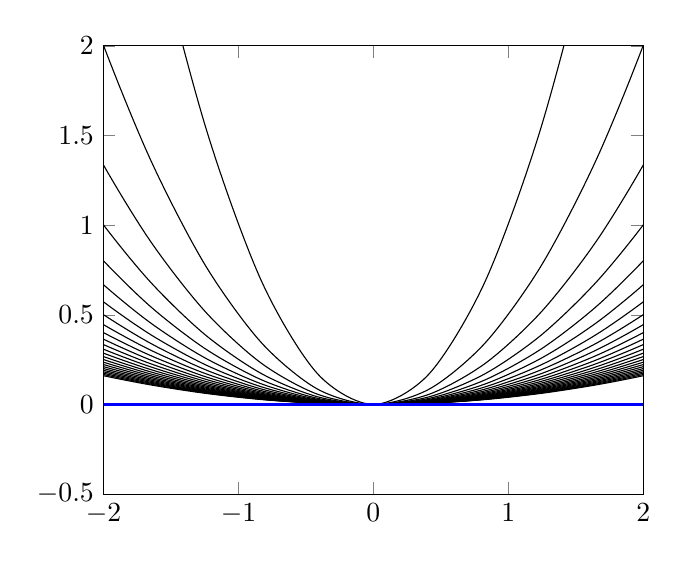
\begin{tikzpicture}[scale=1]
      \begin{axis}[ymin=-0.5, ymax=2, xmin=-2, xmax=2]
        \foreach \i in {1,...,25}
        {\addplot[smooth,domain=-5:5]{x^2/\i};}
        \addplot[domain=-5:5,color=blue,thick]{0};
      \end{axis}
    \end{tikzpicture}
    \caption{ $f_{1}$ tot $f_{25}$ en de nulfunctie }
  \end{figure}
  \extra{bewijs puntsgewijze convergentie}

  \begin{proof}
    Kies $\epsilon = 1$ en een willekeurige $n_{0} \in \mathbb{N}$.
    Kies een $x \ge \sqrt{n_{0}}$ en $n = n_{0}$, dan geldt het volgende:
    \[ \frac{1}{n}x^{2} \ge \frac{1}{n_{0}}\left(\sqrt{n_{0}}\right)^{2} = 1 \ge \epsilon \]
  \end{proof}
\end{vb}

\begin{st}
  \label{str:uniform-dan-puntsgewijs}
  Een rij functies $(f_{n})_{n}$ die uniform convergeert, convergeert puntsgewijs.
\extra{bewijs}
\end{st}

\begin{tvb}
  Een rij functies $(f_{n})_{n}$ die puntsgewijs convergeert, convergeert niet noodzakelijk uniform.
\extra{tegenvoorbeeld}
\end{tvb}

\begin{bst}
  Beschouw een rij $(f_{n})_{n}$ van functies $f_{n}: A \subseteq \mathbb{R} \rightarrow \mathbb{R}$ die op $A$ uniform convergeert naar een functie $f:\ A \rightarrow \mathbb{R}$.
  \begin{itemize}
  \item Als $f_{n}$ continu is in een $a\in A$ voor elke $n$, dan is ook $f$ continu in $a$.
  \item Als $f_{n}$ uniform continu is op $A$ voor elke $n$, dan is ook $f$ uniform continu op $A$. 
  \end{itemize}

  \begin{proof}
    Rechtstreeks vanuit de definitie.
    \begin{itemize}
    \item 
      Kies een willekeurige $\epsilon \in \mathbb{R}_{0}^{+}$.
      Omdat $(f_{n})_{n}$ uniform convergeert naar $f$, kunnen we een $n_{0}\in \mathbb{N}$ vinden zodat voor alle $y\in A$ en voor alle volgende $n\in \mathbb{N}$ het volgende geldt:
      \[ |f_{n}(y)-f(y)|<\frac{\epsilon}{3} \]
      Omdat $f_{n}$ continu is in $a$ kunnen we een $\delta$ vinden
      zodat voor alle $x\in A$ uit $|x-a|<\delta$ het volgende geldt:
      \[ |f_{n}(x) - f_{n}(a) < \frac{\epsilon}{3} \]
      Voor elke $x\in A$ met $|x-a|<\delta$ geldt nu het volgende:
      \[
      \begin{array}{rl}
        |f(x)-f(a)| &= |f(x) - f_{n}(x) + f_{n}(x) - f_{n}(a) + f_{n}(a) - f(a)|\\
                    &\le |f(x) - f_{n}(x)| + |f_{n}(x) - f_{n}(a)| + |f_{n}(a) - f(a)|\\
                    &< \frac{\epsilon}{3} + \frac{\epsilon}{3} + \frac{\epsilon}{3}\\
                    &= \epsilon
      \end{array}
      \]
      $f$ is dus continu in $a$.
\extra{hermaken}
    \item
      Kies een willekeurige $\epsilon \in \mathbb{R}_{0}^{+}$.
      \begin{itemize}
      \item Omdat $(f_{n})_{n}$ uniform convergeert naar $f$ kunnen we een $n_{0} \in \mathbb{N}$ vinden zodat het volgende geldt voor alle $x \in A$ en alle $m \ge n_{0}$:
        \[ \forall x\in A, \forall m\ \in \mathbb{N}: m \ge n_{0} \Rightarrow |f(x)-f_{m}(x)| < \frac{\epsilon}{3} \]
      \item 
        Omdat $f_{n}$ uniforum continu is op $A$, kunnen we een $\delta \in \mathbb{R}_{0}^{+}$ vinden als volgt:
        \[ \forall x,y \in A:\  |x-y| < \delta \Rightarrow |f(x)-f(y)| < \frac{\epsilon}{3} \]
      \end{itemize}
      Voor elke $x,y \in A$ met $|x-y| < \delta$ vinden we nu het volgende:
      \[
      \begin{array}{rl}
        |f(x)-f(y)| &= |f(x)-f_{n}(x) + f_{n}(x) - f_{n}(y) + f_{n}(y) - f(y)|\\
                    &\le |f(x)-f_{n}(x)| + |f_{n}(x) - f_{n}(y)| + |f_{n}(ay) - f(y)|\\
                    &< \frac{\epsilon}{3} + \frac{\epsilon}{3} + \frac{\epsilon}{3}\\
                    &= \epsilon
      \end{array}
      \]
      $f_{n}$ is dus uniforum continu op $A$.
    \end{itemize}
  \end{proof}
\end{bst}

\section{Limieten van functies}
\label{sec:limi-van-funct}

\subsection{Het limietbegrip voor functies}

\begin{de}
  Zij $f:\ A \subseteq \mathbb{R} \rightarrow \mathbb{R}$ een functie en $a\in \mathbb{R}$ een ophopingspunt van $A$.
  We noemen de \term{limiet} van $f$ in $a$ ...
  \begin{itemize}
  \item ... $L\in \mathbb{R}$ als het volgende geldt:
    \[
    \lim_{x\rightarrow a}f(x) = L \quad\Leftrightarrow\quad
    \forall \epsilon \in \mathbb{R}_{0}^{+}: \exists \delta \in \mathbb{R}_{0}^{+}: \forall x\in A:\ 0 < |x-a| < \delta \Rightarrow |f(x) - L| < \epsilon
    \]
  \item ... $+\infty$ als het volgende geldt:
    \[
    \lim_{x\rightarrow a}f(x) = +\infty\quad\Leftrightarrow\quad
    \forall M \in \mathbb{R}: \exists \delta \in \mathbb{R}_{0}^{+}: \forall x\in A:\ 0 < |x-a| < \delta \Rightarrow f(x) > M
    \]
  \item ... $-\infty$ als het volgende geldt:
    \[
    \lim_{x\rightarrow a}f(x) = -\infty\quad\Leftrightarrow\quad
    \forall M \in \mathbb{R}: \exists \delta \in \mathbb{R}_{0}^{+}: \forall x\in A:\ 0 < |x-a| < \delta \Rightarrow f(x) < M
    \]
  \end{itemize}
\end{de}

\begin{de}
  Zij $A$ een deelverzameling van $\mathbb{R}$.
  We noemen ...
  \begin{itemize}
  \item ... $+\infty$ een \term{ophopingspunt} van $A$ als het volgende geldt:
    \[ \forall N \in \mathbb{R}:\ A \cap \interval[open right]{N}{+\infty} \neq \emptyset \]
  \item ... $-\infty$ een \term{ophopingspunt} van $A$ als het volgende geldt:
    \[ \forall N \in \mathbb{R}:\ A \cap \interval[open left]{-\infty}{N} \neq \emptyset \]
  \end{itemize}
\end{de}

\begin{de}
  Zij $f:\ A \subseteq \mathbb{R} \rightarrow \mathbb{R}$ een functie en $A \subseteq \mathbb{R}$ zodat $+\infty$ een ophopinspunt is van $A$.
  We noemen de \term{limiet} van $f$ in $+\infty$ ...
  \begin{itemize}
  \item ... $L\in \mathbb{R}$ als het volgende geldt:
    \[
    \lim_{x\rightarrow +\infty}f(x) = L \quad\Leftrightarrow\quad
    \forall \epsilon \in \mathbb{R}_{0}^{+}: \exists N \in \mathbb{R}: \forall x\in A:\ x > N \Rightarrow |f(x) - L| < \epsilon
    \]
  \item ... $+\infty$ als het volgende geldt:
    \[
    \lim_{x\rightarrow +\infty}f(x) = +\infty\quad\Leftrightarrow\quad
    \forall M \in \mathbb{R}: \exists N \in \mathbb{R}: \forall x\in A:\ x > N \Rightarrow f(x) > M
    \]
  \item ... $-\infty$ als het volgende geldt:
    \[
    \lim_{x\rightarrow +\infty}f(x) = -\infty\quad\Leftrightarrow\quad
    \forall M \in \mathbb{R}: \exists N \in \mathbb{R}: \forall x\in A:\ x > N \Rightarrow f(x) < M
    \]
  \end{itemize}
\end{de}

\begin{de}
  Zij $f:\ A \subseteq \mathbb{R} \rightarrow \mathbb{R}$ een functie en $A \subseteq \mathbb{R}$ zodat $-\infty$ een ophopinspunt is van $A$.
  We noemen de \term{limiet} van $f$ in $-\infty$ ...
  \begin{itemize}
  \item ... $L\in \mathbb{R}$ als het volgende geldt:
    \[
    \lim_{x\rightarrow -\infty}f(x) = L \quad\Leftrightarrow\quad
    \forall \epsilon \in \mathbb{R}_{0}^{+}: \exists N \in \mathbb{R}: \forall x\in A:\ x > N \Rightarrow |f(x) - L| < \epsilon
    \]
  \item ... $+\infty$ als het volgende geldt:
    \[
    \lim_{x\rightarrow -\infty}f(x) = +\infty\quad\Leftrightarrow\quad
    \forall M \in \mathbb{R}: \exists N \in \mathbb{R}: \forall x\in A:\ x < N \Rightarrow f(x) > M
    \]
  \item ... $-\infty$ als het volgende geldt:
    \[
    \lim_{x\rightarrow -\infty}f(x) = -\infty\quad\Leftrightarrow\quad
    \forall M \in \mathbb{R}: \exists N \in \mathbb{R}: \forall x\in A:\ x < N \Rightarrow f(x) < M
    \]
  \end{itemize}
\end{de}

\begin{bpr}
  \label{pr:limiet-van-functie-asa-limiet-van-beeld-van-rij}
  Beschouw een functie $f:\ A \subseteq \mathbb{R} \rightarrow \mathbb{R}$ en een $L \in \mathbb{R} \cup \{-\infty,+\infty\}$.
  Zij $a \in \mathbb{R} \cup \{-\infty,+\infty\}$ een ophopingspunt van $A$.
  De limiet van $f(x)$ in $a$ is $L$ als en slechts als $L$ ook de limiet is van het beeld van elke rij $(x_{n})_{n}$ in $A\setminus\{a\}$ die $a$ als limiet heeft.

  \begin{proof}
    Gevalsonderscheid.
    \begin{itemize}
    \item $a = -\infty$
      \begin{itemize}
      \item $L = -\infty$
\extra{bewijs}
      \item $L \in \mathbb{R}$
\extra{bewijs}
      \item $L = +\infty$
\extra{bewijs}
      \end{itemize}
    \item $a\in\mathbb{R}$
      \begin{itemize}
      \item $L = -\infty$
\extra{bewijs}
      \item $L \in \mathbb{R}$
        \begin{itemize}
        \item $\Rightarrow$
          Zij $(x_{n})_{n}$ een rij in $A\setminus \{a\}$ met $a$ als limiet.
          Kies een willekeurige $\epsilon \in \mathbb{R}_{0}^{+}$.
          Omdat de limiet van $f$ in $a$ $L$ is, bestaat er dan een $\delta \in \mathbb{R}_{0}^{+}$ zodat uit voor alle $x\in A$ uit $|x-a|<\delta$ volgt dat $|f(x)-L|<\epsilon$ geldt.
          Omdat de rij convergeert naar $a$, bestaat er een $n_{0}\in \mathbb{N}$ zodat voor alle volgende $n\in\mathbb{N}$ geldt dat $|x_{n}-a|$ kleiner is dan $\delta$.
          Vanaf die $n_{0}$ is $|f(x_{n})-L|$ dus kleiner dan $\epsilon$.
        \item $\Leftarrow$
        \end{itemize}
      \item $L = +\infty$
\extra{bewijs}
      \end{itemize}
    \item $a = +\infty$
      \begin{itemize}
      \item $L = -\infty$
\extra{bewijs}
      \item $L \in \mathbb{R}$
\extra{bewijs}
      \item $L = +\infty$
\extra{bewijs}
      \end{itemize}
    \end{itemize}
  \end{proof}
\end{bpr}

\begin{de}
  Zij $f:\ A \subseteq \mathbb{R} \rightarrow \mathbb{R}$ een functie en $a\in \mathbb{R}$.
  \begin{itemize}
  \item Als $a$ een ophopingspunt is van $\interval[open left]{-\infty}{a} \cap A$ zeggen we dat $f$ een \term{linkerlimiet} heeft in $a$ als de beperking van $f$ tot $\interval[open left]{-\infty}{a} \cap A$ een limiet $L \in \mathbb{R} \cup \{ -\infty, +\infty \}$ heeft.
    \[ \lim_{x \overset{<}{\rightarrow} a}f(x) = L \quad\text{of}\quad \lim_{x \rightarrow a^{-}}f(x) = L \quad\text{of}\quad f(a^{-}) = L \]
  \item Als $a$ een ophopingspunt is van $\interval[open right]{a}{+\infty} \cap A$ zeggen we dat $f$ een \term{rechterlimiet} heeft in $a$ als de beperking van $f$ tot $\interval[open right]{a}{+\infty} \cap A$ een limiet $L \in \mathbb{R} \cup \{ -\infty, +\infty \}$ heeft.
    \[ \lim_{x \overset{>}{\rightarrow} a}f(x) = L \quad\text{of}\quad \lim_{x \rightarrow a^{+}}f(x) = L \quad\text{of}\quad f(a^{+}) = L \]
  \end{itemize}
\end{de}

\begin{st}
  Een equivalente definities voor een linker- en rechterlimiet.\\
  Zij $f:\ A \subseteq \mathbb{R} \rightarrow \mathbb{R}$ een functie en $a\in\mathbb{R}$ een ophopingspunt van $A$.
  \begin{itemize}
  \item De linker limiet van $f$ in $A$ noemen we $L$ als het volgende geldt:
    \[ \forall \epsilon\in\mathbb{R}_{0}^{+},\ \exists \delta \in \mathbb{R}_{0}^{+}:\ \forall x\in A:\ a-\delta<x\le a \Rightarrow |f(x)-L|<\epsilon \]
  \item De rechter limiet van $f$ in $A$ noemen we $L$ als het volgende geldt:
    \[ \forall \epsilon\in\mathbb{R}_{0}^{+},\ \exists \delta \in \mathbb{R}_{0}^{+}:\ \forall x\in A:\ a\le x < a+\delta \Rightarrow |f(x)-L|<\epsilon\]
  \end{itemize}
  \extra{bewijs}
\end{st}

\subsection{Classificatie van discontinuiteiten}

\begin{bpr}
  \label{pr:functie-continu-asa-limiet-is-beeld}
  Zij $f:\ A \subseteq \mathbb{R} \rightarrow \mathbb{R}$.
  Stel dat $a$ zowel een element van $A$ als een ophopingspunt van $A$ is.
  $f$ is continu in $a$ als de limiet van $f$ in $a$ $f(a)$ is.

  \begin{proof}
    $f$ is continu in $a$, dus voor elke rij $(x_{n})_{n}$ in $A$ die naar $a$ convergeert geldt dat $(f(x_{n}))_{n}$ naar $f(a)$ convergeert.\prref{pr:continu-asa-behoudt-convergentie}
    Dit is equivalent met de stelling dat $f(a)$ de limiet is van $f$ in $a$.\prref{pr:limiet-van-functie-asa-limiet-van-beeld-van-rij}
  \end{proof}
\end{bpr}

\begin{bpr}
  Zij $f:\ A \subseteq \mathbb{R} \rightarrow \mathbb{R}$ en $a\in \mathbb{R}$.
  Stel dat $a$ een ophopingspunt is van zowel $\interval[open right]{a}{+\infty} \cap A$ als $\interval[open left]{-\infty}{a} \cap A$.
  $f$ heeft in $a$ een limiet $L\in \mathbb{R}\cup \{ -\infty,+\infty\}$ als en slechts als de linker- en rechterlimiet van $f$ in $a$ bestaan en gelijk zijn aan $L$.

  \begin{itemize}
  \item $\Rightarrow$\\
    \extra{bewijs}
  \item $\Leftarrow$\\
    Stel dat $f$ zowel een linker- als een rechterlimiet heeft in $a$ en ze beide gelijk zijn aan $L$.
    Kies dan een willekeurige $\epsilon\in\mathbb{R}_{0}^{+}$.
    Er bestaat dan een $\delta_{l}$ en een $\delta_{r}$ als volgt.
    \[ \forall x\in A:\ a-\delta_{l}<x\le a \Rightarrow |f(x)-L|<\epsilon \]
    \[ \forall x\in A:\ a\le x < a+\delta_{r} \Rightarrow |f(x)-L|<\epsilon \]
    Noem nu $\delta = \min\{\delta_{1},\delta_{2}\}$ zodat het volgende geldt.
    \[ \forall x\in A:\ a\le |x-a|<\delta \Rightarrow |f(x)-L|<\epsilon \]
    $f$ heeft dus $L$ als limiet in $a$.
  \end{itemize}
\end{bpr}

\begin{de}
  Beschouw een functie $f:\ A \subseteq \mathbb{R} \rightarrow \mathbb{R}$ en $a\in A$.
  Stel dat $f$ niet continu is in $a$, dan karakteriseren we deze discontinu\"eteit als volgt:
  \begin{itemize}
  \item Als de limiet van $f$ naar $a$ bestaat en eindig is, noemen we $a$ een \term{ophefbare discontinu\"iteit}.
  \item Als $a$ een ophopingspunt is van zowel $\interval[open right]{a}{+\infty} \cap A$ als $\interval[open left]{-\infty}{a} \cap A$ en als zowel de linker als de rechterlimiet van $f$ in $a$ bestaan, maar ze zijn niet gelijk, dan noem men $a$ een \term{discontinu\"iteit van de eerste soort} of \term{sprongdiscontinu\"iteit}.
  \item Als $a$ een ophopingspunt is van $\interval[open left]{-\infty}{a} \cap A$, maar de limiet van $f$ in $a$ niet bestaat, of als $a$ een ophopingspunt is van $\interval[open right]{a}{+\infty}$, maar de limiet van $f$ in $a$ niet bestaat, dan noemt men $a$ een \term{discontinu\"iteit van de tweede soort} of \term{essentie\"ele discontinu\"iteit}.
  \end{itemize}
\end{de}

\begin{bpr}
  Zij $f:\ I \subseteq \mathbb{R} \rightarrow \mathbb{R}$ een monotone functie op een (niet-leeg) open interval $I$, dan kan $f$ enkel discontinu\"iteiten van de eerste soort vertonen.
  Bovendien is het aantal discontinu\"iteiten van $f$ aftelbaar.

  \begin{proof}
    Gevalsonderscheid:
    \begin{itemize}
    \item $f$ is monotoon stijgend.
      \begin{itemize}
      \item De linkerlimiet van $f$ in elk punt $a\in I$ bestaat en is eindig
        Die linkerlimiet wordt in het bijzonder gegeven als volgt:
        \[ \lim_{x \overset{<}{\rightarrow} a}f(x) = \sup\{ f(x)\mid x\in I \wedge x < a \} \]
        De verzameling $\{ f(x)\mid x\in I \wedge x < a \}$ is immers een niet-lege, naar boven begrensde verzameling.
        Noem $s$ het supremum van die verzameling.
        Kies een willekeurige $\epsilon \in \mathbb{R}_{0}^{+}$, dan
        bestaat er een $y\in I$ groter dan $a$ zodat $f(y)$ tussen
        $s-\epsilon$ en $s$ ligt.  Omdat $f$ stijgt, zal voor alle
        $x\in F$ tussen $y$ en $a$ gelden dat $f(x)$ tussen $f(y)$ en
        $s$ ligt.  Noem nu $\delta = a-y > 0$.  Voor alle
        $x\in I\cap\interval[open left]{-\infty}{a}$ met
        $0<|x-a|<\delta$ geldt dan dat $|f(x)-s|<\epsilon$ geldt.
      \item De rechterlimiet van $f$ in elk punt $a\in I$ bestaat en is eindig.
        Die rechterlimiet wordt in het bijzonder gegeven als volgt:
        \[ \lim_{x \overset{>}{\rightarrow} a}f(x) = \inf\{ f(x)\mid x\in I \wedge x > a \} \]
      \item Vermits de linker- en rechterlimiet van $f$ in elk punt van $I$ bestaan, kunnen we al besluiten dat $f$ enkel discontinu\"iteiten van de eerste soort kan hebben.
      \item Merk op dat de linkerlimiet kleiner of gelijk aan de rechterlimiet is in elk punt $a\in I$.
        Als en slechts als de limieten verschillend zijn is $f$ niet continu in $a$.
        (Omdat $f$ monotoon stijgt kan er geen ophefbare discontinu\"iteit zijn.)
        De verzameling $D$ van de discontinu\"iteiten van $f$ ziet er dus als volgt uit:
        \[ D = \left\{ a \in I \mid \lim_{x \overset{<}{\rightarrow} a}f(x)- \lim_{x \overset{>}{\rightarrow} a}f(x) > 0 \right\} \]
        We tonen aan dat $D$ afterlbaar is.\\
        Merk eerst op dat voor $k$ elementen $a_{i}$ uit $D$ tussen $c$ en $d$ in $I$ het volgende geldt:
        \[ \sum_{i=1}^{k}\left(\lim_{x \overset{<}{\rightarrow} a}f(x)- \lim_{x \overset{>}{\rightarrow} a}f(x)\right) \le f(d) - f(c) \]
        Omdat $I$ open is, kunnen we een strikt dalende rij $(c_{n})_{n}$ en een strikt stijgende rij $(d_{n})_{n}$ in $I$ nemen zodat $I$ de unie is van alle intervallen $\interval[open]{c}{d}$.
        Beschouw nu voor elk $n$ de deelverzameling $D_{n}$ van $D$.
        \[ D_{n} = \left\{ a \in \interval[open]{c_{n}}{d_{n}} \mid \left(\lim_{x \overset{<}{\rightarrow} a}f(x)- \lim_{x \overset{>}{\rightarrow} a}f(x)\right) > \frac{1}{n} \right\} \]
        Elke afstand $\left(\lim_{x \overset{<}{\rightarrow} a}f(x)- \lim_{x \overset{>}{\rightarrow} a}f(x)\right)$ is groter dan $\frac{1}{n}$, de som is dus groter dan $\frac{\#D_{n}}{n}$.
        De som is echter ook kleiner dan $f(d_{n})-f(c_{n})$, om tot de volgende ongelijkheid te komen.
        \[ \#D_{n} \le n(f(d_{n})-f(c_{n})) \]
        $\#D_{n}$ is dus eindig.
        $D$ is een aftelbare unie van eindige verzamelingen $D_{n}$ en daarom aftelbaar.
      \end{itemize}
    \item $f$ is monotoon dalend.\\
      \extra{bewijs}
    \end{itemize}
  \end{proof}
\end{bpr}


\subsection{Eigenschappen en rekenregels voor limieten}
\label{sec:eigensch-en-rekenr}

\begin{bpr}
  Beschouw functies $f,g:\ A \subseteq \mathbb{R} \rightarrow \mathbb{R}$ en zij $a\in \mathbb{R} \cup \{-\infty,+\infty\}$ een ophopingspunt van $A$.
  Stel dat $\forall a\in A: f(x) \le g(x)$ geldt, en dat de limiet van zowel $f$ als $g$ in $a$ bestaat, dan is de limiet van $f$ in $a$ kleiner dan of gelijk aan de limiet van $g$ in $a$.\
\extra{bewijs}
\end{bpr}

\begin{bst}
  De \term{insluitstelling voor functies}\\
  Beschouw functies $f,g,h:\ A \subseteq \mathbb{R} \rightarrow \mathbb{R}$ en zij $a\in \mathbb{R} \cup \{-infty,+\infty\}$ een ophopingspunt van $A$.
  Stel dat $\forall a\in A: f(x) \le g(x) \le h(x)$ geldt, en dat de limiet van zowel $f$ als $h$ in $a$ bestaat en deze gelijk zijn, dan bestaat de limiet van $g$ in $x$ en zijn de drie limieten gelijk.
\extra{bewijs}
\end{bst}

\begin{bpr}
  Beschouw functies $f,g:\ A \subseteq \mathbb{R} \rightarrow \mathbb{R}$ en zij $a\in \mathbb{R} \cup \{-infty,+\infty\}$ een ophopingspunt van $A$.
  Zij $\lambda \in \mathbb{R}$ en stel dat de limieten van $f$ en $g$ in $a$ bestaan en eindig zijn.
  \begin{itemize}
  \item $\lim_{a}(\lambda f) = \lambda \lim_{a} f$
  \item $\lim_{a}(f+g) = \lim_{a}f + \lim_{a}g$
  \item $\lim_{a}(fg) = \lim_{a}f \lim_{a}g$
  \item $\lim_{a}\frac{f}{g} = \frac{\lim_{a}f}{\lim_{a}g}$ als $\lim_{a}g \neq 0$ met $\frac{f}{g}:\ \{x\in A\mid g(x) \neq 0\} \rightarrow \mathbb{R}:\ x \mapsto \frac{f(x)}{g(x)}$
  \end{itemize}
\extra{bewijs}
\end{bpr}

\extra{zelfde extra rekenregels voor oneindigheden etc (veel werk)}

\begin{bpr}
  Beschouw functies $f:\ A \subseteq \mathbb{R} \rightarrow B \subseteq \mathbb{R}$ en $g:\ B \rightarrow \mathbb{R}$.
  Zij $a\in \mathbb{R} \cup \{-infty,+\infty\}$ een ophopingspunt van $A$.
  Stel dat de limiet $b$ van $f$ in $a$ bestaat.
  \begin{itemize}
  \item Als $b$ in $B$ zit en $g$ continu is in $b$, dan bestaat de limiet van $g\circ f$ in $a$:
    \[ \lim_{a}g\circ f = g(\lim_{a}f) \]
  \item Als $b$ niet tot $B$ behoort, dan is $b$ een ophopingspunt van $B$ en de limiet van $g$ in $b$ bestaat, dan bestaat de limiet van $g\circ f$ in $a$:
    \[ \lim_{a}g\circ f = \lim_{a}g \]
  \end{itemize}

  \begin{proof}
    Gevalsonderscheid
    \begin{itemize}
    \item
      Kies een willekeurige rij $(x_{n})_{n}$ in $A\setminus\{a\}$ die naar $a$ convergeert.
      We bewijzen dat $((g\circ f)(x_{n}))_{n}$ naar $(g\circ f)(a)$ convergeert.
      Hieruit volgt dan de stelling.\prref{pr:limiet-van-functie-asa-limiet-van-beeld-van-rij}
      Omdat $b$ de limiet is van $f$ in $a$ weten we dat $(f(x_{n})_{n}$ een rij is die naar $b$ convergeert.
      Omdat $g$ continu is in $b$ geldt dan het volgende:
      \[ \lim_{n\rightarrow \infty}(g\circ f)(x_{n}) = \lim_{n\rightarrow \infty}g(f(x_{n})) = g(b) \]
      Hiermee is het volgende aangetoond:
      \[ \lim_{a}(g\circ f)=g(b) \]
    \item \extra{bewijs}
    \end{itemize}
  \end{proof}
\end{bpr}

\begin{bst}
  Zij $(f_{n})_{n}$ een rij van functies van $A \subseteq \mathbb{R}$ naar $\mathbb{R}$ die uniform op $A$ convergeert naar een functie $f: A \rightarrow \mathbb{R}$.
  Zij $a\in \mathbb{R} \cup \{-\infty,+\infty\}$ een ophopingspunt van $A$.
  Stel dat voor alle $n$ de limiet $L_{n}$ van $f_{n}$ in $a$ bestaat en eindig is.
  \[ \lim_{a}f = \lim_{n \rightarrow +\infty} L_{n} = \lim_{n\ \rightarrow +\infty} \lim_{x \rightarrow a} f_{n}(x) \]

  \begin{proof}
    Bewijs in delen.
    \begin{itemize}
    \item $(L_{n})_{n}$ is een Cauchyrij.
      Kies een willekeurige $\epsilon \in \mathbb{R}_{0}^{+}$.
      Omdat $(f_{n})_{n}$ uniform op $A$ convergeert kunnen we een $n_{0}\in \mathbb{N}$ vinden zodat het volgende geldt:
      \clarify{mag dit zomaar? extra bewijs maken: cauchyrij van functies!}
      \[ \forall x\in A:\ \forall n,m \ge m_{0}:\ |f_{n}(x) -f_{m}(x)| < \epsilon \]
      Door van deze ongelijkheid de limiet te nemen voor $x$ gaande naar $x$ vinden we de volgende ongelijkheid:
      \clarify{mag dit zomaar?}
      \[ \forall n,m \ge m_{0}:\ |L_{n}-L_{m}| \le \epsilon \]
      Dit toont dat $(L_{n})_{n}$ een Cauchyrij is.
      Omdat $\mathbb{R}$ volledig is zal dan $(L_{n})_{n}$ convergeren.
      We noteren de limiet met $L$.
    \item 
      Kies nu een willekeurige rij $(x_{k})_{k} \in A\setminus \{a\}$ die naar $a$ convergeert.
      We zullen bewijzen dat, in de limiet naar $a$, het beeld van $x_{k}$ naar $L$ gaat.
      Merk eerst op dat het volgende geldt:
      \[ \forall k\in \mathbb{N}:\ \forall n\in \mathbb{N}:\ |f(x_{n})-L| \le |f(x_{k}) -f_{n}(x_{k})| + |f_{k}(x_{k})-L_{n}| + |L_{n}-L| \]
      Omdat $(L_{n})_{n}$ naar $L$ convergeert kunnen we een $n_{0}\in\mathbb{N}$ nemen zodat het volgende geldt voor alle volgende $n\in \mathbb{N}$:
      \[ |L_{n}-L| < \frac{\epsilon}{3} \]
      Omdat $(f_{n})_{n}$ uniform convergeert op $A$ naar $f$, kunnen we een $n_{1}\in \mathbb{N}$ nemen zodat het volgende geldt voor alle volgende $n\in \mathbb{N}$:
      \[ \forall x\in A:\ |f_{n}-f(x)| < \frac{\epsilon}{3} \]
      Omdat $(f_{n}(x_{k}))_{k}$ voor alle $n$ naar $L_{n}$ convergeert (omdat $f$ continu is), kunnen we een $k_{0} \in \mathbb{N}$ vinden zodat ook het volgende geldt voor alle volgende $k \in \mathbb{N}$:
      \[ |f_{n}(x_{k}) - L_{n}| < \frac{\epsilon}{3} \]
      Noem nu $n' = \max\{n_{0},n_{1},k_{1}\}$, dan geldt voor alle volgende $n\in \mathbb{N}$ de bewering die de stelling bewijst:
      \[ |f(x_{n})-L| \le |f(x_{k}) -f_{n}(x_{k})| + |f_{k}(x_{k})-L_{n}| + |L_{n}-L| < \frac{\epsilon}{3} + \frac{\epsilon}{3} + \frac{\epsilon}{3} = \epsilon \]
    \end{itemize}
  \end{proof}
\end{bst}












\end{document}

%%% Local Variables:
%%% mode: latex
%%% TeX-master: t
%%% End:
